\documentclass[12pt,a4paper,bibliography=totoc,listof=totoc]{scrartcl}
% u.U. muss Koma-Skript Package ueber MikTeX deinstalliert und neu installiert werden
% Hilft das nicht, so sollte statt scrartcl die Dokumentenklasse article verwendet werden
\usepackage[ngerman]{babel}
\usepackage[utf8]{inputenc}
\usepackage{ifthen}
\usepackage{xargs}
\usepackage{amsmath}
\usepackage{amsfonts}
\usepackage{amssymb}
\usepackage{graphicx}
\usepackage{fancyhdr}
\usepackage{tabularx}
\usepackage{geometry}
\usepackage{setspace}
\usepackage[right]{eurosym}
\usepackage[printonlyused]{acronym}
\usepackage{subfig}
\usepackage{floatflt}
\usepackage{float}
\usepackage[usenames,dvipsnames]{color}
\usepackage{colortbl}
\usepackage{paralist}
\usepackage{array}
\usepackage{parskip}
\usepackage[right]{eurosym}
\usepackage[subfigure,titles]{tocloft}
\usepackage[pdfpagelabels=true]{hyperref}

\usepackage{listings}
\lstset{basicstyle=\footnotesize, captionpos=b, breaklines=true, showstringspaces=false, tabsize=2, frame=lines, numbers=left, numberstyle=\tiny, xleftmargin=2em, framexleftmargin=2em}
\makeatletter
\def\l@lstlisting#1#2{\@dottedtocline{1}{0em}{1em}{\hspace{1,5em} Lst. #1}{#2}}
\makeatother

\geometry{a4paper, top=35mm, left=35mm, right=25mm, bottom=40mm, headsep=10mm, footskip=10mm}

\definecolor{codered}{rgb}{0.6,0,0} % for strings
\definecolor{codegreen}{rgb}{0.25,0.5,0.35} % comments
\definecolor{codepurple}{rgb}{0.5,0,0.35} % keywords
\definecolor{codeblue}{rgb}{0.25,0.35,0.75} 
\definecolor{codegray}{rgb}{0.6,0.6,0.6}
 
\lstset{language=C,
basicstyle=\ttfamily\footnotesize,
keywordstyle=\color{codepurple}\bfseries,
stringstyle=\color{codered},
commentstyle=\color{codegreen}\itshape\bfseries,
morecomment=[s][\color{codeblue}]{/**}{*/},
numbers=left,
numberstyle=\tiny\color{codegray},
stepnumber=1,
numbersep=10pt,
tabsize=2,
showspaces=false,
showstringspaces=false}


% begin change
%\titlespacing{\section}{0pt}{12pt plus 4pt minus 2pt}{-6pt plus 2pt minus 2pt}
% end change

% Kopf- und Fusszeile
\renewcommand{\sectionmark}[1]{\markright{#1}}
\renewcommand{\leftmark}{\rightmark}
\pagestyle{fancy}
\lhead{}
\chead{}
\rhead{\thesection\space\contentsname}
\lfoot{}
\cfoot{}
\rfoot{\ \linebreak \thepage}
\renewcommand{\headrulewidth}{0.4pt}
\renewcommand{\footrulewidth}{0.4pt}

% Vorspann
\renewcommand{\thesection}{\Roman{section}}
\renewcommand{\theHsection}{\Roman{section}}
\pagenumbering{Roman}

\newcommand{\folgen}[1]{
\ensuremath
#1
}

\newcommandx{\student}[3][]{
	\def\studentName{#1}%
	\def\studentMatnr{#2}%
	\def\studentStudiengang{#3}%
}

\newcommandx{\studentt}[3][]{
	\def\studentNamet{#1}%
	\def\studentMatnrt{#2}%
	\def\studentStudiengangt{#3}%
}


\newcommandx{\studenttt}[3][]{
	\def\studentNamett{#1}%
	\def\studentMatnrtt{#2}%
	\def\studentStudiengangtt{#3}%
}
\newcommandx{\studentttt}[3][]{
	\def\studentNamettt{#1}%
	\def\studentMatnrttt{#2}%
	\def\studentStudiengangttt{#3}%
}
\newcommandx{\studenttttt}[3][]{
	\def\studentNametttt{#1}%
	\def\studentMatnrtttt{#2}%
	\def\studentStudiengangtttt{#3}%
}


\newcommandx{\MyTitelseite}[8][]{
\thispagestyle{empty}
%
\includegraphics[scale=0.2]{pics/oth-logo.png}\hfill\includegraphics[scale=0.2]{#1}

\includegraphics[scale=0.2]{pics/oth-logo.png}
\begin{center}
\ifthenelse{\equal{#2}{2}}{ % then
	\vspace*{2cm}
	\Large
	\textbf{Ostbayerische Technische Hochschule Regensburg}\\
	\textbf{Fakultät für Informatik und Mathematik}\\
	\vspace*{2cm}
	\Huge
	\textbf{#3}\\[1em]
	\large
	%Zur Erlangung des akademischen Grades des\\
	%\ifthenelse{\equal{#3}{Bachelorarbeit}}{Bachelor of Science (B.Sc.)}{Master of Science (M.Sc.)}\\
	\vspace*{1cm}
	\Large
	\textbf{#4}\\
}{ % else
	\vspace*{1cm}
	\Large
	\textbf{#4}\\
	\vspace*{2cm}
	\large
	An der Fakultät für Informatik und Mathematik der\\
	Ostbayerischen Technischen Hochschule Regensburg\\
	im Studiengang\\
	\studentStudiengang\\[2em]
	eingereichte\\
	\vspace*{1cm}
	\Large
	\textbf{#3}\\[2em]
	\large
	%zur Erlangung des akademischen Grades des\\
	%\ifthenelse{\equal{#3}{Bachelorarbeit}}{Bachelor of Science (B.Sc.)}{Master of Science (M.Sc.)}
	\vspace*{1cm}
	\Large
}
	\vfill
	\normalsize
	%\newcolumntype{x}[1]{>{\raggedleft\arraybackslash\hspace{0pt}}p{#1}}
	\begin{tabular}{rl}%{6cm}p{7.5cm}}
	    \rule{0mm}{1ex}\textbf{Name:} & \studentName \\
		\rule{0mm}{1ex}\textbf{Matrikelnummer:} & \hspace*{-0.5em}\begin{tabular}[t]{r}\studentMatnr\end{tabular} \\ 
		\rule{0mm}{1ex}\textbf{Name:} & \studentNamet \\
		\rule{0mm}{1ex}\textbf{Matrikelnummer:} & \hspace*{-0.5em}\begin{tabular}[t]{r}\studentMatnrt\end{tabular} \\ 
		\rule{0mm}{1ex}\textbf{Name:} & \studentNamett \\
		\rule{0mm}{1ex}\textbf{Matrikelnummer:} & \hspace*{-0.5em}\begin{tabular}[t]{r}\studentMatnrtt\end{tabular} \\ 
				\rule{0mm}{1ex}\textbf{Name:} & \studentNamettt \\
		\rule{0mm}{1ex}\textbf{Matrikelnummer:} & \hspace*{-0.5em}\begin{tabular}[t]{r}\studentMatnrttt\end{tabular} \\ 
				\rule{0mm}{1ex}\textbf{Name:} & \studentNametttt \\
		\rule{0mm}{1ex}\textbf{Matrikelnummer:} & \hspace*{-0.5em}\begin{tabular}[t]{r}\studentMatnrtttt\end{tabular} \\ 
		%\ifthenelse{\equal{#2}{1}}{~\\}{\rule{0mm}{1ex}\textbf{Studiengang:} & \studentStudiengang \\[2em]}
		\newline \\
		\rule{0mm}{1ex}\textbf{Erstgutachter:} & #5 \\ 
		\rule{0mm}{1ex}\textbf{Zweitgutachter:} & #6 \\[2em]
		\rule{0mm}{1ex}\textbf{Abgabedatum:} & #7 \\
	\end{tabular} 
	

%\end{center}	
%\end{center}
	
	
\end{center}
\pagebreak
}
\usepackage[utf8]{inputenc}
\usepackage[ngerman]{babel}
\usepackage{subfig}
\begin{document}


% ----------------------------------------------------------------------------------------------------------
% Titelseite
% ----------------------------------------------------------------------------------------------------------
\student{Michael Braun}	% Studierender
{3113161}						% Matrikelnummer
{Technische Informatik}			% Studiengang

\studentt{Korbinian Federholzner}	% Studierender
{3114621}						% Matrikelnummer
{Technische Informatik}			% Studiengang

\studenttt{Philipp Kramer}	% Studierender
{3117284}						% Matrikelnummer
{Technische Informatik}			% Studiengang

\studentttt{Patrick Lesch}	% Studierender
{2917177}						% Matrikelnummer
{Technische Informatik}			% Studiengang

\studenttttt{Michael Schmidt}	% Studierender
{2907322}						% Matrikelnummer
{Technische Informatik}			% Studiengang


%\MyTitelseite{pics/oth-logo-informatik.png}	% Optionales Logo des extern betreuenden Unternehmens
\MyTitelseite{}
{1}								% Style der Titelseite (1 oder 2)
{Projektdokumentation (Datenverarbeitung in der Technik)}			% Typ der Arbeit 
{Balancing Plate}				% Thema der Arbeit						
{Prof.\ Dr.\ Richard Roth}   % Betreuer
{Hr.\ Matthias Altmann}	% Zweitgutachter
{10.2.\the\year}				% Abgabedatum

\setcounter{page}{1} 

%-----------------------------------------------------------------------------------------------------------
% Abstract Zusammenfassung
%-----------------------------------------------------------------------------------------------------------
%\section*{Kurzfassung}
%...
%\pagebreak

%\section*{Abstract}
%...
%\pagebreak

%\section*{Danksagung}
%...
%\pagebreak

% ----------------------------------------------------------------------------------------------------------
% Inhaltsverzeichnis
% ----------------------------------------------------------------------------------------------------------
\tableofcontents
\pagebreak

% ----------------------------------------------------------------------------------------------------------
% Inhalt
% ----------------------------------------------------------------------------------------------------------
% Abstände Überschrift
% begin change
% alte Befehle
%\titlespacing{\section}{0pt}{12pt plus 4pt minus 2pt}{-6pt plus 2pt minus 2pt}
%\titlespacing{\subsection}{0pt}{12pt plus 4pt minus 2pt}{-6pt plus 2pt minus 2pt}
%\titlespacing{\subsubsection}{0pt}{12pt plus 4pt minus 2pt}{-6pt plus 2pt minus 2pt}
% neue Befehle
\RedeclareSectionCommands[
beforeskip=-.9\baselineskip,
afterskip=.4\baselineskip
]{section,subsection,subsubsection}
%end change

% Kopfzeile
\renewcommand{\sectionmark}[1]{\markright{#1}}
\renewcommand{\subsectionmark}[1]{}
\renewcommand{\subsubsectionmark}[1]{}
\lhead{Kapitel \thesection}
\rhead{\rightmark}

%\onehalfspacing
\setstretch{1.15}
\renewcommand{\thesection}{\arabic{section}}
\renewcommand{\theHsection}{\arabic{section}}
\setcounter{section}{0}
\pagenumbering{arabic}
\setcounter{page}{1}

% ----------------------------------------------------------------------------------
% Kapitel 1: Einleitung
% ----------------------------------------------------------------------------------
\section{Einführung/ Projektkontext}

%Grober Inhalt des Lastenhefts in Verbindung mit den Änderungen zur ersten Version (App als Pflicht, 
%keine Rückgabe der Servostellung). 
Der Grundaufbau des Prototyps ist eine Plexiglasplatte, auf der sich 
eine Kugel befindet. Diese Kugel wird durch Druck auf eine resistive Touch-Folie (Wertbestimmung durch 
Druck) erkannt und die zugehörigen Daten werden an einen Raspberry Pi 4 übermittelt. Dieser berechnet dann 
den Offset zum gewünschten Stellpunkt auf der Platte und mit Hilfe eines PID-Reglers die neuen Stellwerte 
für die Servomotoren. Diese Daten werden an einen XMC 4500 übermittelt, welcher die zuvor ermittelten Werte 
in PWM-Signale übersetzt und diese dann an die zuständigen Servomotoren übergibt. Diese bewegen die 
Plexiglasplatte, auf der sich die Touch-Folie befindet, um so die Kugel zu balancieren.
Die Versuchsapparatur soll selbstständig in der Lage sein eine Kugel auf einer Platte in eine vorher 
festgelegte Position, meist die Mitte der Platte, zu manövrieren. Dies soll durch Heben bzw. Senken der 
Plexiglasplatte mittels dreier Servomotoren geschehen. Optional ist dabei die manuelle Steuerung der 
Platte mittels einer App, welche über eine WiFi-Schnittstelle mit dem Raspberry Pi in Verbindung stehen 
soll. Diese App soll dabei das im Handy verbaute Gyroskop verwenden, um den Neigungswinkel des Geräts zu 
erfassen und die Platte dementsprechend zu neigen. Auch eine GUI sollte in der App vorhanden sein.
\newline Im Gegensatz zum Lastenheft, dass kurz nach dem Start abgegeben werden musste, haben sich im 
Laufe des Projektes einige Änderungen ergeben. Dabei wurde die Steuerung mittels einer iOS-App nunmehr 
als Pflichtmodul angesehen. Außerdem wurde das Auslesen der Potentiometer der Servomotoren aus Zeitgründen 
fallengelassen.
\pagebreak
% ----------------------------------------------------------------------------------
% Kapitel 2: Umsetzung
% ----------------------------------------------------------------------------------
\section {Umsetzung}
Um eine konsistente Abarbeitung zu gewährleisten wurde das Projekt in verschieden Module/Arbeitspakete 
geteilt.

\begin{table}[]
\centering
\begin{tabular}{|l|l|l|l|}
\hline
Name 					& Aufgabe 1 			& Aufgabe 2 				& Aufgabe 3  \\
\hline
Michael Braun			& Physischer Aufbau		& Reglerentwicklung			& PWM-Signale \\
\hline
Korbinian Federholzner	& Ansteuerung mit App	& UART Schnittstelle		& Touch-Folie \\
\hline
Philipp Kramer			&Reglerentwicklung		& Modellerstellung Matlab	& Touch-Folie\\
\hline
Patrick Lesch			& Ansteuerung mit App	& WiFi Schnittstelle		& Custom Kernel\\
\hline
Michael Schmidt			& Physischer Aufbau		& UART Schnittstelle		& PWM-Signale\\
\hline
\end{tabular}
\label{tab:Arbeisverteilung}
\caption{Arbeisverteilung}
\end{table}

Diese werden immer von mindestens zwei Projektteilnehmern abgearbeitet. Außerdem wurde auf eine in sich 
geschlossene Aufteilung geachtet, um bei aneinandergrenzenden Modulen immer einen Ansprechpartner zu haben. 
Um durch eine gegenseitige Kontrolle eine funktionierende Version sicherzustellen und um eine 
Qualitätskontrolle durchzuführen, wurden in dem Git-Repository die Funktion push-Requests aktiviert.
\pagebreak
% ----------------------------------------------------------------------------------
% Kapitel 2.1: Physischer Bau
% ----------------------------------------------------------------------------------
\subsection{Physicher Aufbau}
\textit{Von Michael Braun und Michael Schmidt}\newline

\subsubsection {Mechanik}

\begin{figure}[htbp]
	\centering
	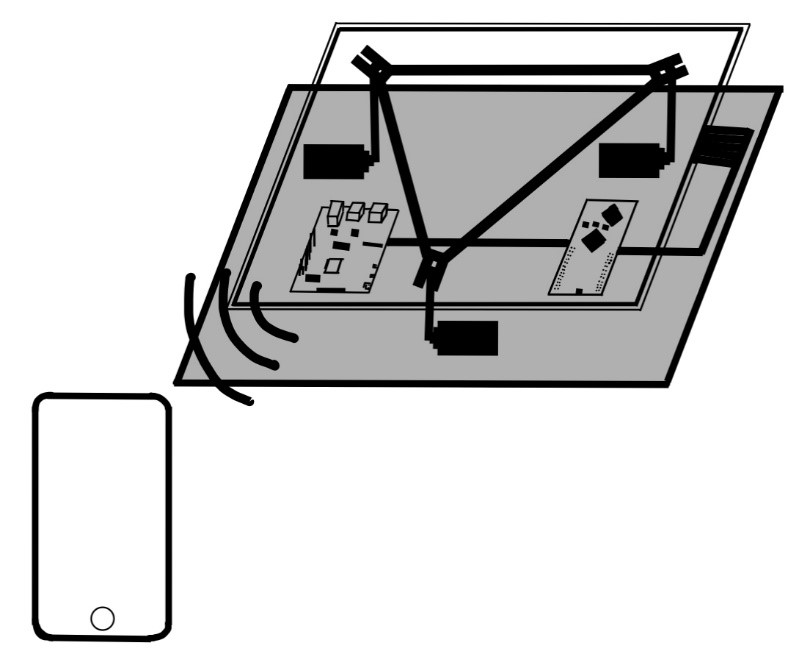
\includegraphics[scale = 0.9]{pics/SkizzeAufbau}
	\caption{Skizzierter Aufbau des Prototypen}
	\label{fig:Skizze}
\end{figure}

In \ref{fig:Skizze} ist eine Skizze des physischen Aufbaus aus dem Lastenheft zum Start des Projektes zu 
sehen. Dabei wurde lediglich graphisch eine mögliche Vorversion des späteren Prototyps gezeichnet. 

\begin{figure}[htbp]
	\centering
	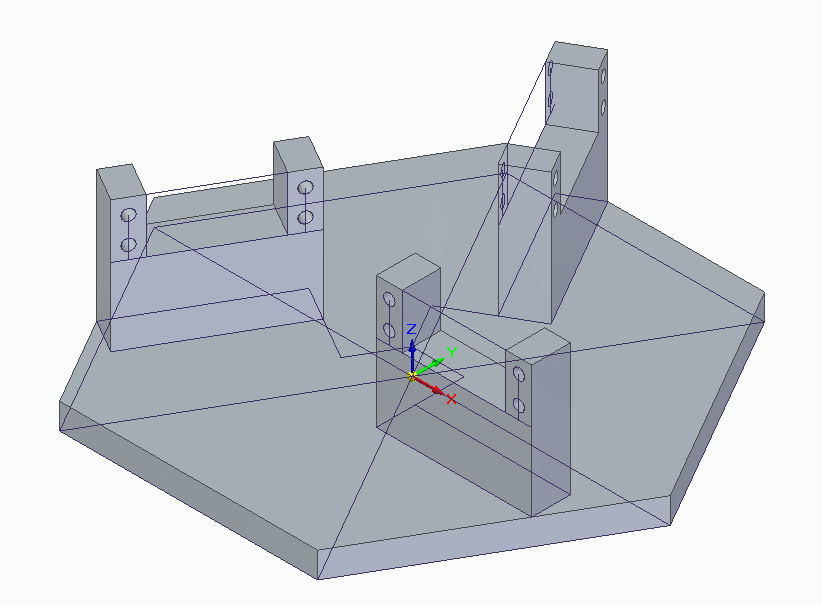
\includegraphics[scale = 0.45]{pics/BildGrundplatte}
	\caption{Grundplatte des Prototypen}
	\label{fig:Grundplatte}
\end{figure}

Im Gegensatz zu \ref{fig:Skizze} wurde eine sechseckige Grundplatte mit den Halterungen für die drei 
Servomotoren mittels Solid Edge 2020 konstruiert und mittels eines 3D-Druckers gefertigt. Diese ist 
in \ref{fig:Grundplatte} zu sehen

Der Druck der Grundplatte dauerte dabei etwa zehn Stunden, was unter anderem an den Ausmaßen der Platte 
(Durchmesser von 20 cm) liegt. Nachdem die Servomotoren in den Halterungen befestigt wurden, hat man die 
Servo-Hebel und Gabelköpfen verbunden, dazu wurden die Servo-Hebel aufgebohrt. Nach dem Zusammenbau hat man 
festgestellt, dass zwischen den Hebeln und dem Gabelkopf noch zu viel Spielraum war, der die Regelung 
beeinträchtigen könnte. Deshalb wurden Unterlegescheiben zur Verringerung des Spiels eingesetzt. Die 
Verbindung zur Platte wird über ein Dreieckskonstrukt \ref{fig:Dreiecksverbindung}, das ebenfalls aus dem 
3D-Drucker kam, hergestellt. 

\begin{figure}[htbp]
	\centering
	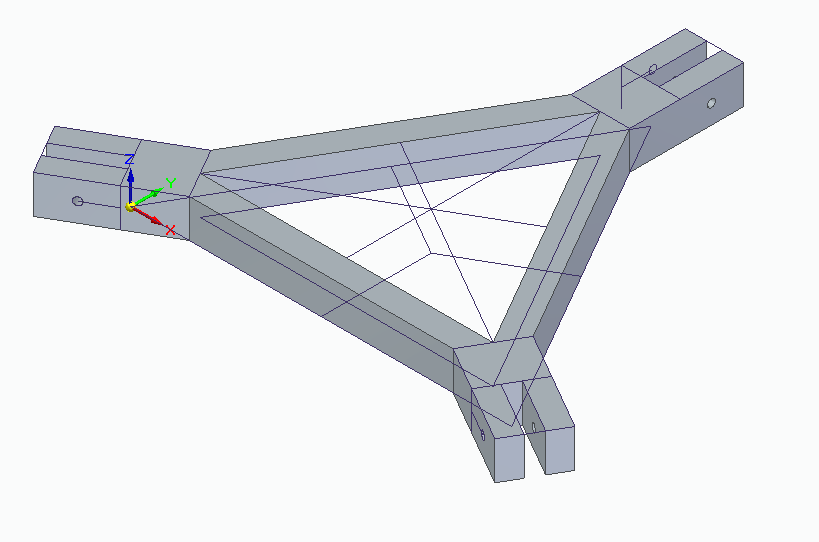
\includegraphics[scale = 0.45]{pics/BildDreieck}
	\caption{Dreiecksverbindung zur Touch-Folie}
	\label{fig:Dreiecksverbindung}
\end{figure}

Dabei war vor allem die korrekte Länge zum Mittelpunkt des Dreiecks, 
respektive der Grundplatte, eine wichtige Größe, da eine falsche Länge nicht mehr die senkrechte 
Ausrichtung des Gabelkopfes zu der Grundplatte zur Folge gehabt hätte. Außerdem mussten die Kugellager 
passend in den Gabelkopf der Dreiecksverbindung eingefügt werden, um eine seitliche Drehung dieser zu 
verhindern.
Der 3D-Druck dieser Verbindung dauerte in etwa sechs Stunden. Die Konstruktion dieser beiden Bauteile 
nahm in etwa fünfzehn Stunden in Anspruch. Diese Dreieckskonstruktion liegt genau über dem markierten 
Dreieck der Grundplatte. Die Touch-Folie befindet sich dabei auf einer Plexiglasplatte, welche mittels 
Silikon mit der Dreiecksverbindung zusammengefügt wurde.
Außerdem wurden vor dem Zusammenbau der Servomotoren mit den Servo-Hebeln, alle Servomotoren in die 
Neutralstellung gesetzt (vgl. PWM-Signale), um die Regelung ebenfalls von einem neutralen Punkt aus zu 
starten. Dabei traten motorspezifische Unterschiede auf die mittels der PWM-Werte ausgeglichen werden 
müssen.

\subsubsection{Schaltplan und Verkabelung}

\begin{figure}[htbp]
	\centering
	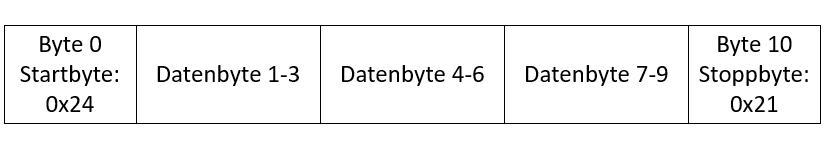
\includegraphics[scale = 0.5]{pics/Schaltplan}
	\caption{Schaltplan des Prototyps}
	\label{fig:verkabelung}
\end{figure}
Die gesamte Verkabelung ist dabei in \ref{fig:1verkabelung} zu sehen. Hier sind auch alle Pins verzeichnet, 
sollte sich einmal ein Kabel lösen. Dabei wurde die Stromversorgung für den XMC und den Raspberry Pi getrennt 
von der allgemeinen Stromversorgung für die Servomotoren gehalten, um ein Absacken der Spannung zu verhindern.

\subsubsection{Fazit}
Die Teile aus dem 3D-Drucker waren insgesamt sehr zufriedenstellend, lediglich die Löcher für die Schrauben 
an der Dreiecksverbindung mussten nachträglich aufgebohrt werden. Dasselbe galt für die Löcher in den Servohebeln. 
Außerdem blieben von einem Gabelkopf der Dreiecksverbindung leider nicht funktionsessentielle Teile an der Platte 
des Druckers hängen, somit war lediglich der ästethische Punkt beeinträchtigt. Glücklicherweise waren die 
Servomotoren ausreichend stark um die Platte ohne Probleme und mit einer ausreichenden Geschwindigkeit bewegen zu 
können. Des Weiteren wurde aufgrund von Zeitmangel die Verkabelung des Prototypen und die Halterung des Bildschirms 
lediglich provisorisch ausgeführt. An dieser Stelle wäre für zukünftige Projekte noch Verbesserungspotential. 
Insgesamt liegt jedoch ein für unsere Zwecke einfacher und dennoch ausreichender physischer Aufbau vor.

% ----------------------------------------------------------------------------------
% Kapitel 2.2: Software-Architektur
% ----------------------------------------------------------------------------------
\subsection{Software-Architektur}
\begin{figure}[htbp]
	\centering
	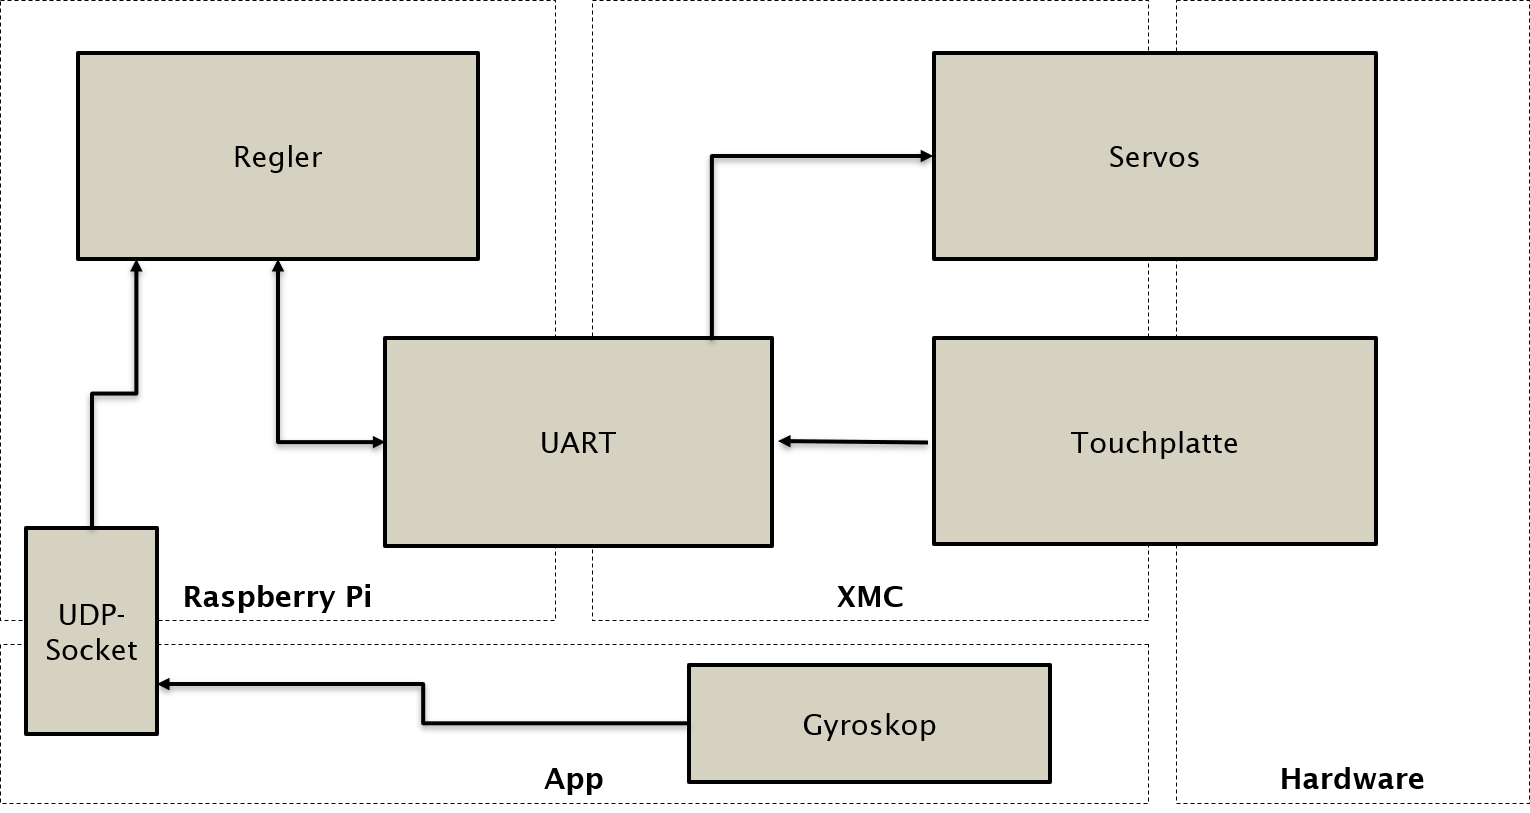
\includegraphics[scale = 0.5]{pics/SW_Architektur}
	\caption{Grundaufbau der Software-Architektur}
	\label{fig:SWarchitektur}
\end{figure}

Wie in \ref{fig:SWarchitektur} zu sehen gliedert sich der Aufbau der Software in drei Teile. Zum einen der 
Programmteil auf dem XMC, der die eingehenden Daten verarbeitet und an die Servomotoren weiterleitet und 
gleichzeitig die Werte der Touch-Platte ausliest. Zum zweiten die Regelung auf dem Raspberry Pi, welche 
die ankommenden Werte von der Touchplatte umwandelt und an den XMC zurücksendet. Außerdem beschäftigt sich 
dieser Teil mit dem Threading zwischen den beiden Modi: Steuerung mittels App und selbstständige Regelung.  
Für die Steuerung per App müssen auch hier die ankommenden Daten verarbeitet werden. Die App bildet dabei 
den dritten Teil in dem die eingebauten Gyroskope des Handys ausgelesen und diese Werte an den Raspberry Pi 
übermittelt werden.
% ----------------------------------------------------------------------------------
% Kapitel 2.3: Touch-Folie
% ----------------------------------------------------------------------------------
\subsection{Touch-Folie} \label{subsec:Touch-Folie}
\textit{Von Korbinian Federholzner und Philipp Kramer}\newline

Nachdem feststand, dass dieses Projekt ein Balancing Plate sein wird, war einer der ersten Schritte die Suche nach vergleichbaren selbstbalancierenden Platten, um nachzusehen, welche Hardware diese verwenden. Hauptsächlich relevant war dafür, wie die einzelnen Vergleichsprojekte die Position des Balles erkennen können. Eine der am beiden am meisten vertretenen Aufbauten war es, eine einfache Plastikplatte zu verbauen und den Ball mithilfe einer Kamera zu erkennen. Diese Umsetzung war aufgrund von mangelnder Kenntnis in der Bildverarbeitung und dem Ziel, das Endprodukt so simpel und kompakt wie möglich zu gestalten, allerdings nicht die letztendliche Wahl. Die Entscheidung fiel dafür eine Touch-Folie zu nutzen und mit einer ausreichend schweren Kugel per Druck die Koordinaten zu bestimmen. Da die Suche nach einer geeigneten Platte auf den deutschen Markt eingegrenzt war, war es schwerer als erwartet eine passende Touch-Platte zu finden. Endgültig fiel die Entscheidung auf das in Abb. \ref{fig:bestell} genannte Platte AMT 2517 der Apex Material Technology Corp.

\subsubsection{Funktion der Touch Folie}

\begin{figure}[htbp]
	\centering
	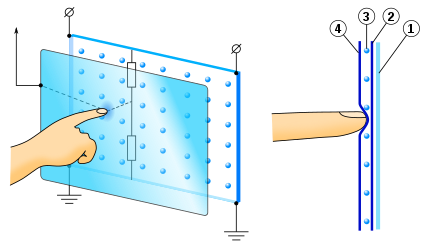
\includegraphics[scale = 0.6]{pics/TouchScreen_5wires.png}
	\caption{Funktion des Touch Panels} 
	\label{fig:TouchPanelFunction}
\end{figure}

Zum Auslesen der Sensorwerte wird ein 5-Wire rezessives Touch Panel verwendet.\newline
Wie in Abb. \ref{fig:TouchPanelFunction} \cite {wikipdeia} gezeigt, besteht dieses grundsätzlich aus zwei Schichten. Wird ein Druck von 1.00 $Newton$ oder mehr auf die Oberfläche des Panels ausgeübt, so berühren sich die beiden Schichten. Da das Touch Panel im Prinzip ein Spannungsteiler ist, ergeben sich, je nachdem wo gedrückt wird, unterschiedliche Widerstände, welche wiederum einen Rückschluss geben auf die Position des Druckpunktes. Der analoge Spannungswert, der durch Pin 3 zurückgegeben wird, ist also durch diesen Spannungsteiler bestimmt.\newline
Um zu messen, wo auf der Touchplatte sich ein Druckpunkt befindet, werden zwei der fünf Pins des Panels auf Masse (GND) gesetzt und zwei auf Spannung (V\textsubscript{DD}), im Fall dieses Projektes sind dies 5 $Volt$. Die Verwendung von fünf Kabeln bietet den Vorteil, dass der Pin in der Mitte, Pin 3, zum Auslesen des analogen Sensorwerts verwendet wird.
Sind wie in Abb. \ref{fig:TouchPanelFunction} die oberen beiden Pins auf V\textsubscript{DD} und die unteren beiden auf GND, so lässt sich ermitteln, wo der Druckpunkt sich zwischen der oberen und der unteren Kante befindet. Bei einem kartesischen zweidimensionalen Koordinatensystem entspricht dies dem y-Wert.
Da mit dieser Methode nur eine Richtung gemessen werden kann, für einen Punkt auf dem Panel allerdings sowohl ein y- als auch ein x-Wert benötigt wird, müssen die Pins so umgeschaltet werden, sodass beide Pins an der linken kurzen Seite auf V\textsubscript{DD} sind und beide Pins auf der rechten Seite GND.\newline
Die Werte der Platte liegen bei perfekten Bedingungen zwischen  0 und 4096, wobei 0 an der Kante, an der GND anliegt, ist und 4096 der maximale Wert an der V \textsubscript{DD}-Seite. Bei diesem Projekt liegen die Werte, die letztlich ausgegeben werden, bei beiden Seiten zwischen 1500 und 2500. Die Verringerung der Anzahl der Messwerte ist zum Teil auf die in Kapitel \ref{subsec:ProblemePlatte} angeführten Probleme zurückzuführen.

\subsubsection{Implementierung}

\begin{figure}[htbp]
	\centering
	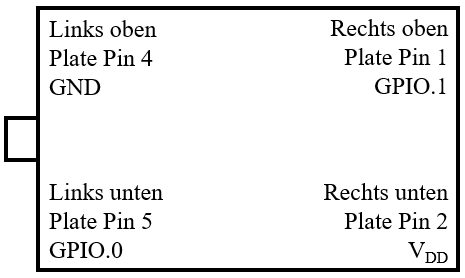
\includegraphics[scale = 0.6]{pics/PlatteSkizze.png}
	\caption{Skizze der Platte} 
	\label{fig:PlatteSkizze}
\end{figure}

Bei der Implementierung wird als Verbindung zur Touch Plate ein XMC4500 Mikrocontroller verwendet, welcher mit der Applikation Dave4 der Infineon AG programmiert wird.
Die einzelnen Pins der Platte sind hierbei mit Pins des XMC verbunden. Da, wie in \ref{subsec:Touch-Folie} beschrieben, die Pins an der Platte umgeschaltet werden müssen, um sowohl x-, als auch y- Koordinate auslesen zu können, werden zwei GPIO-Pins des XMC verwendet. Bei einem skizzierten Aufbau der Platte wie in Abb. \ref{fig:PlatteSkizze} werden die Pins 1 und 5 mit GPIO-Pins des XMC verbunden. Pin 1 und Pin 5 müssen immer jeweils gegenteilig sein, also wenn Pin 1 high ist, ist Pin 5 low und vice versa.
Der übrige Pin 3 wird ausschließlich dafür verwendet die Werte, die die Platte liefert, in je eine x-Variable und eine y-Variable zu schreiben. 
In diesem Projekt sind die Pins der Touch Plate wie in Tabelle \ref{tab:VerbindungenPins} mit dem XMC verbunden.

\begin{table}[]
\centering
\begin{tabular}{l|l}
Pin Touch Plate & Pin XMC \\
\hline
Pin 1           & Pin 2.15\\
Pin 2           & VDD     \\
Pin 3           & Pin 15.2    \\
Pin 4           & GND     \\
Pin 5           & Pin 2.14
\end{tabular}
\caption{Verbindungen der Pins der Touch Plate mit dem XMC \label{tab:VerbindungenPins}}
\end{table}

Da das Panel nur mit einer Frequenz von 50 Hz geschaltet werden kann, also alle 0.02 Sekunden, ist ein Timer-Interrupt definiert. Dieser wird alle 20 ms ausgelöst, das Panel wird also maximal oft ausgelesen. Die Interrupt Service Routine (ISR) startet die Messung für den Analog Digital Converter (ADC). Dieser ADC wandelt die analoge Spannung, die per Pin 3 der Touch Plate an den XMC geleitet wird, in einen digitalen Wert um, der, wie bereits in Kapitel \ref{subsec:Touch-Folie} beschrieben, zwischen 1500 und 2500 liegt. Sobald der ADC die Messung und Umwandlung abgeschlossen hat, startet er selbst ebenfalls eine 
Der ADC löst sobald er mit dem Messen fertig ist auch eine ISR aus. In dieser wird der gemessene digitale Wert je nach gemessener Koordinate in eine x- bzw. y-Variable gespeichert und daraufhin die GPIO Pins umgeschaltet, sodass die andere Koordinate ermittelt werden kann.
Die GPIO-Pins sind beim Start des Programms so eingestellt, dass erst der x-Wert ausgelesen wird und daraufhin der y-Wert. Sind beide Werte vorhanden, so wird bei beiden Variablen jeweils 1500 abgezogen. Dadurch sind die weiterverwendeten nicht mehr im Bereich von 1500 bis 2500, sondern befinden sich zwischen 0 und 1000, was die darauffolgenden Berechnungen erleichtert. Nach der Umrechnung werden die beiden Daten in einem UART Frame verpackt und dann ein UART-Transmit ausgelöst.
Der gesamte Ablauf ist schematisch in Abb. \ref{fig:TouchUML} dargestellt.

\begin{figure}[htbp]
	\centering
	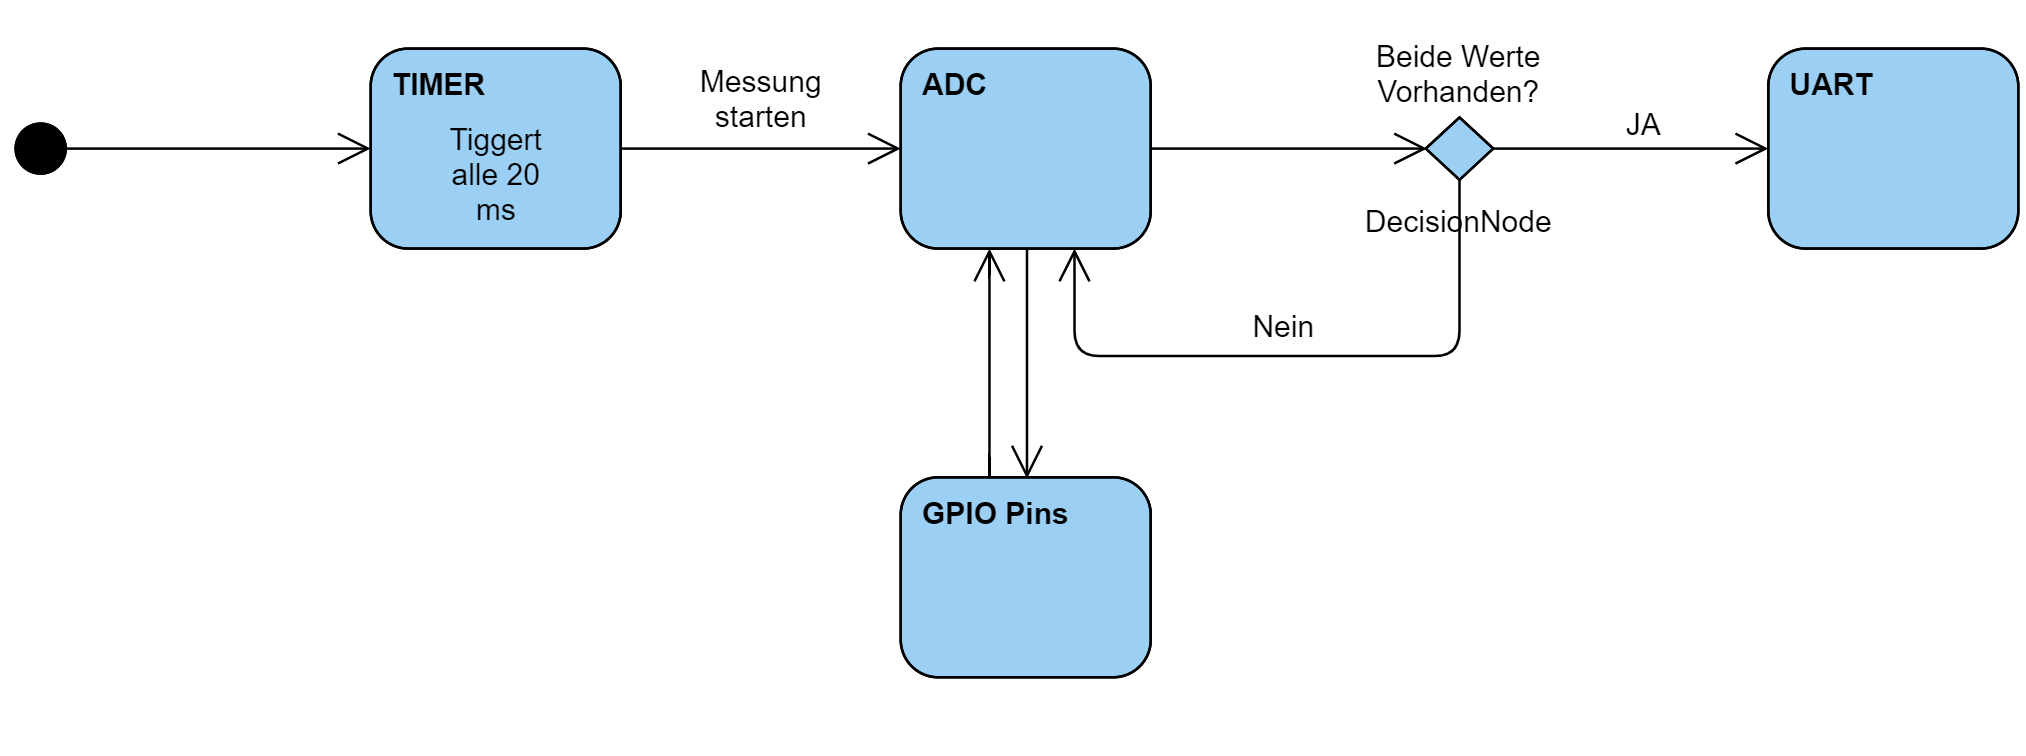
\includegraphics[scale = 0.6]{pics/TouchUML.png}
	\caption{UML Aktivitätsdiagramm der Interrupts}
	\label{fig:TouchUML}
\end{figure}

\subsubsection{Probleme} \label{subsec:ProblemePlatte}
Ein Problem im Zuge der Implementierung der Touch-Platte war die Funktion der ADC-App im Dave4. Da bei dieser keine gute Dokumentation vorhanden war, war es z.B. schwer herauszufinden, wie sich eine Messung bei dem Analog Digital Converter starten lässt und wie die dafür benötigte Funktion heißt. \newline
Eine weitere Problematik stellt der Randbereich der Platte dar. Dieser ist minimal höher als der Rest der Touch-Folie und auf diesem schwanken die Werte sehr stark. Anstatt eines erwarteten Wertes, der kleiner als 500 ist, werden dort teils Werte von über 2000 ausgegeben. Zur Behebung des Hindernisses wurde ein etwas kleinerer Innenbereich definiert und sollte ein Druckpunkt zwischen dem inneren Bereich und dem etwas erhöhten Rand sein, so wird die Platte maximal ausgelenkt, sodass sich der Ball möglichst wieder in Richtung Mitte der Platte bewegt.
Das Hauptproblem, das bei der Implementierung der Platte anfiel, waren konstante Messfehler des Touch Panels. Das erwartete Verhalten ist, dass die x-Werte konstant bleiben, wenn sich die Druckpunkte parallel zur y-Achse bewegen. Dies entspricht beim endgültigen Aufbau einer Kugelbahn, die parallel zur kurzen Seite verläuft. Plausiblerweise wird das gleiche Verhalten auch bei den y-Werten erwartet, wenn die Druckpunkte parallel zur x-Achse liegen.
Bei Tests stieg allerdings der konstant erwartete Wert entlang der Achsen immer weiter an. In Abb. \ref{fig:ProblemPlattenwerte} ist dieses Verhalten für die Messung des x-Werts dargestellt.
\begin{figure}[htbp]
	\centering
	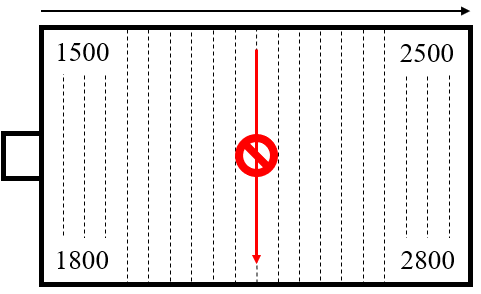
\includegraphics[scale = 0.5]{pics/ProblemPlattenwerte}
	\caption{Problem der Plattenwerte am Beispiel der x-Werte}
	\label{fig:ProblemPlattenwerte}
\end{figure}

Nachdem die Touch Plate mittels eines Picoscopes auf Fehler untersucht war, dort aber alles wie erwartet funktionierte, wurden alle Pins des XMC auf eventuelle Mängel untersucht. Dort waren ebenfalls keine Fehler zu erkennen.\newline
Der nächste Lösungsansatz war es die GPIO-Pins zu eliminieren, indem eine H-Brücke eingesetzt wird. Hintergrund dieser Idee war es, dass die GPIO-Pins des XMC keine wirklich konstante Spannung liefern können und mittels der H-Brücke der Strom nicht mehr vom Mikrocontroller, sondern direkt von der Stromversorgung kommt. Allerdings fiel wie bei den GPIO-Pins des XMC über die H-Brücke die Spannung ab, was zu einem sehr ähnlichen Endszenario führte. Die nächste Überlegung war die Verwendung von Relais. Da Relais, die schnell genug für die Anforderungen dieses Projektes sind, sehr teuer sind und weiterhin deren Verschleiß hoch ist, wurde diese Idee letztlich ebenfalls nicht angewandt.\newline
Die Lösung, die letztendlich im Projekt verwendet wird, ist, Widerstände von 100 $Ohm$ zwischen die Pins des XMC und die der Platte zu schalten. Diese Widerstände minimieren den Fehler so weit, dass er entlang einer Achse nur noch etwa 40 ist und damit vernachlässigbar. Der minimale Fehler, der übrig bleibt, kann außerdem mithilfe des Reglers ausgeglichen werden.
Mit der Kenntnis, dass dieser Ansatz den erhofften Erfolg brachte, lag der Fehler weniger an der mangelnden Konstanz der GPIO-Pins, sondern eher am zu geringen Widerstand, den die Platte liefert, was wiederum zu gelegentlichen Spannungsabbrüchen führte.\newline
Ein anderes Problem, das im Laufe der Tests aufkam, war, dass die erste Kugel, die genutzt wurde, zu leicht war, wenn sich die Platte zu schnell bewegte. Dies war der Fall, da in dem kurzen Moment, in dem sich die Platte bewegte, der Mindestdruck von 1 $Newton$ unterschritten wurde und dadurch falsche Werte an den XMC gesendet wurden. Daraufhin berechnete der Regler neue Plattenneigungswinkel, die allerdings basierend waren auf den unkorrekten Positionen. Eine geeignete Kugel war dann eine Flipperkugel, die der Inhaber der Flipperwerkstatt Regensburg zur Verfügung stellte.


% ----------------------------------------------------------------------------------
% Kapitel 2.4: Einrichtung des Raspberry Pi
% ----------------------------------------------------------------------------------
\subsection{Einrichtung des Raspberry Pi}
\textit{Von Patrick Lesch}
\subsubsection{Allgemeines}
Aufgrund seiner Vielzahl von flexibel einsetzbaren Komponenten wurde der Raspberry Pi 4 als zentraler Bestandteil des Systems gewählt.
Besonders die hohe Rechenleistung sowie das bereits verbaute Wlan-Modul und die einfache Bedienbarkeit waren hierbei ausschlaggebend. 
Als Betriebssystem wurde eine Aktuelle Version des Raspbian Buster Lite gewählt welches ein leichtgewichtiges Image ohne Grafische Oberfläche darstellt.
Die Wahl viel auf dieses Image da hierfür der im anschließenden Kapitel erwähnte Preempt-RT Kernel existiert. Zudem wird keine Rechenleistung
für das Darstellen von Grafiken und Animationen aufgewendet die eventuell die Geschwindigkeit von kritischen Prozessen negativ beeinflussen.
\subsubsection{Echtzeit Preempt-RT Kernel} \label{subsec:Kernel}
\begin{figure}[htbp]
    \centering
    \subfloat[Standard Raspbian Kernel\newline(4.19.57-v7l+)]{{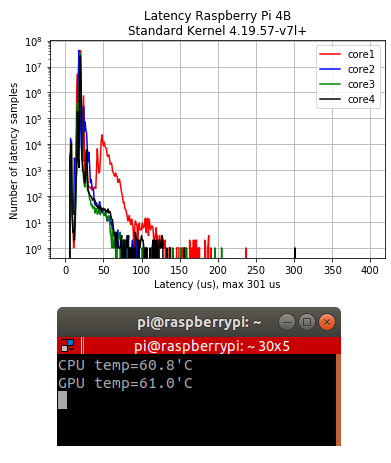
\includegraphics[scale = 0.55]{pics/RaspiKernelBefore} }}%
    \qquad
    \subfloat[Preempt-RT Raspbian Kernel\newline(4.19.59-rt23-v7l+)]{{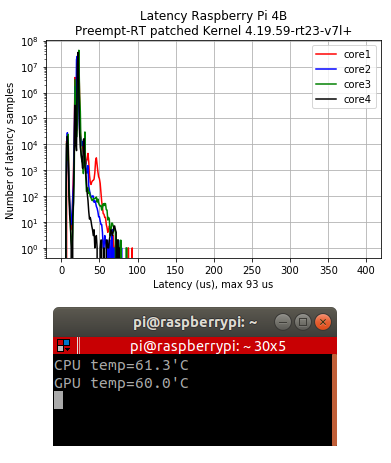
\includegraphics[scale = 0.55]{pics/RaspiKernelAfter} }}%
    \caption{Latenzen und Temperaturen der jeweiligen Kernel}%
    \label{fig:Kernel}%
\end{figure}
Um die Echtzeitfähigkeit des gesamten Systems zu optimieren wurde für den Raspberry Pi der Preempt-RT Kernel kompiliert und aufgespielt.
Die Latenzen verbessern sich in Tests, wie in Abbildung \ref{fig:Kernel} zu sehen ist, 
um einen Faktor von 3 während die Temperatur der CPU um nur 0.5$^\circ$ C steigt. Dies stellt objektiv betrachtet eine
Verhältnismäßig gute Kosten-Nutzen Balance dar.
\subsubsection{Ausblick}
Auch wenn das Potential des Preempt-RT Kernels aktuell nicht voll ausgeschöpft wird bietet er das Potential künftige Funktionalität auf einem 
möglichst schnellen Level zu halten wodurch die Echtzeitfähigkeit des Systems gewährleistet wird.

% ----------------------------------------------------------------------------------
% Kapitel 2.5: UART Schnittstelle
% ----------------------------------------------------------------------------------
\subsection{UART Schnittstelle}
\textit{Von Korbinian Federholzner und Michael Schmidt}\newline
\subsubsection{Funktion}
\begin{figure}[htbp]
	\centering
	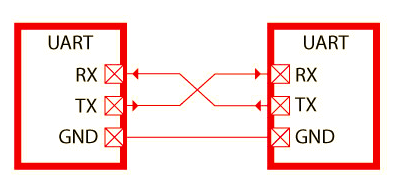
\includegraphics[scale = 0.6]{pics/BildUart1}
	\caption{Grundaufbau der UART-Verbindung} 
	\label{fig:UART}
\end{figure}
Zur Datenübertragung zwischen dem Raspberry Pi und dem XMC Mikrocontroller wurde das Universal 
Asynchronous Receiver Transmitter-Protokoll (UART) verwendet. Dieses ist für schnelle Bitübertragungsraten, 
in unserem Fall eine Baud-Rate von 19200 (Bits pro Sekunde), über eine einzelne Leitung verantwortlich. 
In unserem Fall ist die Übertragung im Modus Full-Duplex und erfordert somit zwei Leitungen, die sich 
kreuzen \ref{fig:UART} \cite {mikroe}.

Grundsätzlich erfolgt die Datenübertragung aufgrund der Einfachheit in Strings, welche jeweils nach dem 
Empfang dekodiert werden. Dabei enthält ein UART-Paket genau ein Zeichen der Zeichenfolge. Ein solches 
Beispielpaket ist in \ref{fig:UARTFrame} zu sehen.Die Übertragung erfolgt dabei auf dem Raspberry Pi über 
die General Purpose In/Out Pins 14 und 15. Dabei ist der Pin 14 der Sender und der Pin 15 der Empfänger 
von den Nachrichten des XMC. Auf dem XMC ist die Pinbelegung variabel und somit flexibler im Gegensatz 
zum Raspberry Pi. Hier wurden die beiden Pins 1.4 und 1.5 gewählt. Hier fungiert Pin 1.5 als Sender und 
Pin 1.4 als Empfänger.
\subsubsection {Testen und erste Fehler}
Zum Testen wurde vom Raspberry Pi ein vordefinierter String, in diesem Fall 
"`\$123456789!",, an den XMC gesendet. Dieser liest die ankommenden Daten und sendet sie zurück an den 
Raspberry Pi, welcher sie auf dem Bildschirm ausgibt. Dadurch ließen sich die nachfolgenden Fehler in 
der Implementierung und Datenverarbeitung des XMC besser nachvollziehen. Am Anfang des Projektes traten diverse Schwierigkeiten 
beim Testen der Implementierung auf. Zum Beispiel war das Flashen des Programmes auf den XMC unmöglich, 
da ein Fehler generiert wurde, da keine Verbindung zu dem auf dem XMC integrierten Debugger hergestellt 
werden konnte. Nach einem Test mit einem anderem XMC gleicher Bauart wurde festgestellt, dass unser erster 
XMC lediglich defekt war. Nach einem Tausch des verwendeten XMC konnte die Programmierung wieder 
fortfahren, allerdings wurden durch diesen Fehler insgesamt ca. 10 Stunden Arbeitszeit in die Fehlersuche 
investiert. Dieses Problem behinderte auch das Arbeitspaket "`PWM-Signale".
Ein weiteres Problem, auf das wir gestoßen sind, war ein Fehler in der Interrupt-Funktion. Auf dem XMC 
lassen sich unter Dave4 in den zur Verfügung gestellten APPs diverse Empfangs- und Sendeoptionen festlegen. 
Darunter war auch das Empfangen mittels eines Interrupts. Dieses Interrupt wurde jedoch beim Testen nicht 
aufgerufen und somit die ankommenden Daten nicht aus dem Speicher ausgelesen. Um dieses Problem zu umgehen 
wurde mittels der Dave4-APP NVIC/Interrupt ein Hardwareinterrupt konfiguriert, welches bei einer Änderung 
des Buses von logisch 0 auf logisch 1 ausgelöst wird und die ankommenden Daten verarbeitet. Dabei traten 
jedoch weitere Probleme auf, wie z.B. die ankommenden Daten waren nicht vollständig, da das Interrupt zu 
schnell ausgelöst wurde und die verbleibenden Daten nicht in den Buffer geschrieben wurden, oder das erste 
Zeichen wurden als "`0" \,interpretiert. Dies hatte folgenden Grund: Das Interrupt wurde zu langsam geöffnet 
und im Buffer kam es zu einem Overflow, sodass die ersten Werte bereits wieder mit "`0"\, überschrieben wurde, 
welche das UART-Protokoll als Byte-Stream-Ende interpretiert und somit nicht korrekte Daten liefert.
Nach intensiver Suche in der integrierten Dokumentation in Dave 4, welche jedoch erst nach einigem Suchen 
gefunden wurde, stießen wir auf eine Funktion:\, "`UART\_StartRecieveIRQ"\,, deren Implementierung anscheinend 
erforderlich war, um mittels der in der UART-APP vorprogrammierten Interrupt-Option die ankommenden Daten 
auszulesen \cite {infineon}
. Diese Funktion setzt einen Interrupt-Request und muss 
kontinuierlich nach dem erstmaligen Empfangen ausgeführt werden, um eine fehlerfreie Abarbeitung zu 
gewährleisten. Somit wird sie nach jedem Empfangsvorgang auf dem XMC in der Interrupt-Routine neu 
aufgerufen.

\subsubsection{Datenübertragungsformate}

Um eine eindeutige Übertragung zu gewährleisten, wurde sich auf ein standardisiertes Format festgelegt. 
Dabei wurden eine bestimmte Anzahl Pakete in einer bestimmten Reihenfolge gesendet, wobei pro Paket immer 
ein Zeichen des Strings übertragen wird, wie in \ref{fig:UARTFrame} \cite {electricimp} verdeutlicht wird.
\begin{figure}[htbp]
	\centering
	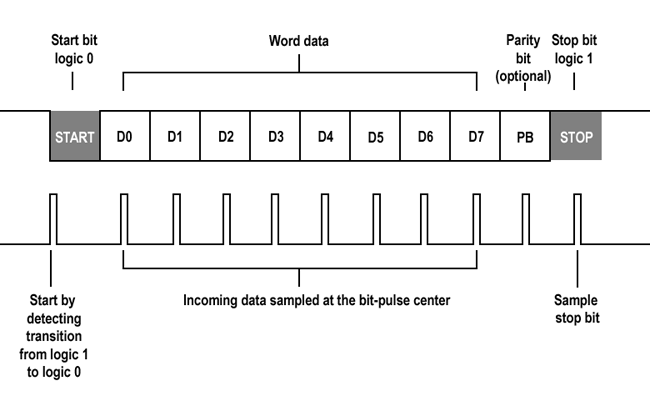
\includegraphics[scale = 0.5]{pics/Uartframe}
	\caption{Aufbau eines UART-Frames}
	\label{fig:UARTFrame}
\end{figure}
Diese Zeichen werden dann aneinandergereiht und ergeben die unten beschriebenen Formate. Dabei hat die 
Kommunikation, bei der der Raspberry Pi der Sender und der XMC 4500 der Empfänger ist folgendes Format 
\ref{fig:UART Servo}.
\begin{figure}[htbp]
	\centering
	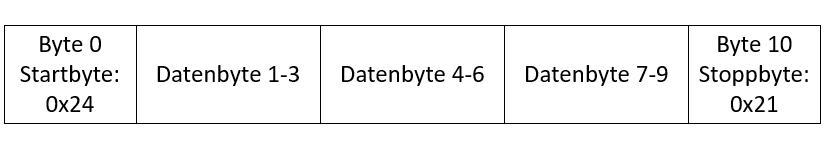
\includegraphics[scale = 0.5]{pics/Uartservo}
	\caption{Aufbau eines Datenpakets mit Servowerten}
	\label{fig:UART Servo}
\end{figure}
Übertragen werden hierbei die aktuellen Werte für die PWM-Signalgenerierung, deren Werte sich zwischen 
450 und 1050 befinden. Dies ist durch die maximale Auslenkung der Servomotoren begründet. Um weitere Bytes 
zu sparen wird nur der Offset von dem Grundwert 450 übermittelt. Dieser wird in einer nachfolgenden 
Funktion wieder dekodiert und in die jeweiligen Variablen gespeichert, auf die die PWM-Signalgenerierung 
zugreift. Dabei befinden sich in den ersten drei Zeichen des Datenteils (Byte 1-3) die Werte für den ersten 
Servomotor., in den zweiten drei (Byte 4-6) die Werte für den zweiten Servomotor und in den letzten drei 
(Byte 6-9) die Werte für den dritten Servomotor, wie in der Abbildung 6 dargestellt. Das Startbyte 0, 
"`0x24"\, und das Stoppbyte 10 "`0x21"\, dienen dabei der Erkennung der feststehenden Feldlänge, um eine korrekte 
und vollständige Übermittlung zu gewährleisten. Die Kommunikation zwischen XMC 4500 und dem Raspberry Pi 
erfolgt über mehrere Formate, da wir mehrere unterschiedliche Nachrichten auf dem Raspberry Pi verarbeiten 
müssen. Zum einen wären da die Übertragung der X- und Y-Koordinaten der Touch-Folie und zum anderen die 
Rückgabewerte der Potentiometer aus den Servomotoren. Um zwischen den beiden Nachrichtentypen, die 
unterschiedliche Längen und Formate haben zu unterscheiden haben wir eine Nachrichten-Identifikationsnummer 
(Message-ID) eingeführt, welche vor den jeweiligen Dekodierungsfunktionen überprüft wird. Lediglich der 
Datenteil unterscheidet sich zwischen den beiden Typen. Da sie als String übertragen werden, ist das 
System problemlos auf bis zu 100 unterschiedliche Nachrichtenformate erweiterbar. Um das bestehende System 
zu erweitern muss lediglich eine zugehörige Dekodierungsfunktion auf dem Raspberry Pi programmiert werden 
und ein korrekter Sendevorgang auf dem XMC sichergestellt werden. Die Nachricht mit den Werten der 
%Touch-Folie hat die Message-ID "`00" \,und wird wie folgt übertragen \ref{fig:UART Platte}.
%\begin{figure}[htbp]
%	\centering
%	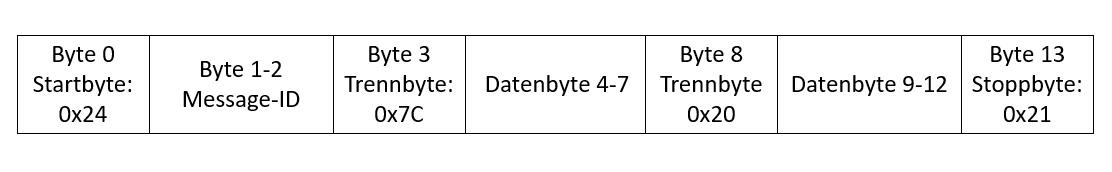
\includegraphics[scale = 0.5]{pics/Uartplatte}
%	\caption{Aufbau eines Datenpakets mit den Werten der Touch-Folie}
%	\label{fig:UART Platte}
%\end{figure}
Auch hier sind Start und Ende der Nachricht wieder mit einem Zeichen, zum Erkennen der korrekten 
Feldlänge, markiert. Dabei werden die Werte der Touch-Folie, die bereits in X-, bzw. Y-Koordinaten 
umgerechnet wurden übertragen. Diese sind in den Datenbytes 4-7 (X-Koordinate) und Datenbytes 9-12 
(Y-Koordinate) kodiert. Zwischen den einzelnen Koordinatenwerten und der Message-ID wurde noch ein 
Trennbyte eingeführt, da die Koordinaten unterschiedliche Länge haben können (3 oder 4 Zeichen). Auf dem 
Raspberry Pi werden diese wieder in integer-Werte umgerechnet und als Koordinaten an die Regelung 
übergeben.
\newline
Allerdings kamen die Formate mit Message-IDs nicht mehr zum Einsatz, da das Auslesen der Servowerte zeitlich 
nicht mehr umgesetzt werden konnte. Daher fallen diese Teilstücke und das nachfolgende Trennbyte aus dem 
Format für die Übertragung der Touch-Plattenwerte heraus. Der Code ist dennoch im Git-Repository vorhanden 
und diese Leitung kann dadurch erweitert werden um multiple Datenformate zu unterstützen.

\subsubsection{CRC-Check}
Da der Austausch der mit UART immer wieder Bit-Errors hatte, gab es immer wieder Störungen an den Servos.
Um die Bitfehler zu erkennen wurde ein CRC-Check implementiert, welcher ein Generatorpolynom über das
gesamte Packet ermittelt. Für die Implementierung wurde eine CRC-Tabelle benutzt, da diese den Vorteil hat,
dass der CRC-Betrag nicht komplett berechnet werden muss, sondern nur ein Teil. Über diesen Anteil kann 
der Wert in der Tabelle nachgeschlagen werden und dieser als CRC-Wert verwendet werden. Der Vorteil einer solchen
Tabelle ist die Performance, da die komplette Rechnung aufwändiger wäre und mehr Performance ziehen würde. Der CRC-Check ist momemtan nur in
der Richtung vom XMC zum Raspberry Pi implementiert, da nur dort die Bit-Errors auftraten. Vom Touch Panel des XMCs zum PI wurde nicht unbedingt ein CRC benötigt,
da auf dem PI ein Kalman-Filter davorgeschalten wurde der diese Fehler ausgleicht. 
In Abbildung \ref{fig:UARTFrameCRC} kann man den geupdateten Frame mit CRC-Check sehen
Der CRC könnte hier in Zukunft noch implementiert werden.
%\begin{figure}[htbp]
%	\centering
%	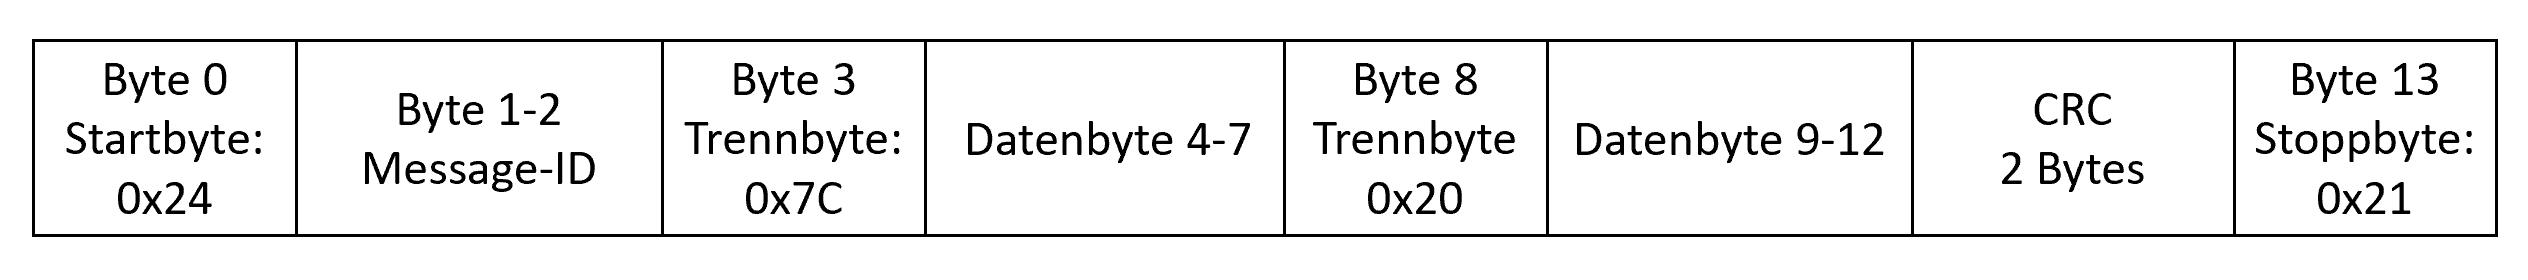
\includegraphics[scale = 0.5]{pics/Uartplattecrc.png}
%	\caption{Aufbau eines Datenpakets mit den Werten der Touch-Folie mit CRC check}
%	\label{fig:UARTFrameCRC}
%\end{figure}
%\subsubsection {Zeitliche Betrachtungen}

Die Übertragungsgeschwindigkeit setzt sich hierbei zusammen aus Baudrate und in unserem Fall Message-Länge:\newline
$\text{Baudrate}/ \text{Message-Länge} = \text {Nachrichtenfrequenz} $\newline
Da in unserem Fall jedoch String-Zeichen und keine einzelnen Bits übertragen werden ergibt sich folgende Frequenz für 
die Nachrichten vom XMC zum Raspberry Pi (Werte der Touch-Platte):\newline
$ 19200/[(10*8)+(10*2)]= 192 \text {Nachrichten pro Sekunde}$\newline
Selbiges ergibt sich für die Nachrichten vom Raspberry Pi zum XMC (Servowerte). Sollte jedoch die Message-ID für die Kommunikation 
von XMC zu Raspberry Pi aktiviert sein ergibt sich durch die geänderte Frame-Länge folgende Rechnung:\newline
$19200 /[(13*8)+(10*2)]=154,8\text {Nachrichten pro Sekunde}$ \newline
Sollte die UART-Verbindung, wie in den beiden Fällen angenommen, vollständig ausgelastet sein, reicht die Verbindung aus um die 
Kommunikation konsistent und vorallem schnell genug zu gewährleisten um eine Regelung zu ermöglichen. Dies liegt daran, dass die 
Servomotoren lediglich in einem 50 Hz Takt arbeiten und die Verbindung somit deutlich schneller arbeitet


\subsubsection{Probleme}
Die größten Probleme beim UART war die Dave4 Dokumentation des XMCs. Online findet man ein sehr detailiertes Handbuch zum 
XMC4500, jedoch nahezu keine Dokumentation wie die enthaltenen Dave4 Apps funktionieren. Die OTH Rechner haben bei der Dave4 IDE keine 
Help Manuals, was das Ganze noch erschwert. Die Lösung dieses Problems war, die Help Manuals auf Dave4 manuell 
nachzuinstallieren. In diesem git es sehr viele nützliche Informationen wie UART eigentlich mittels der App funktioniert und welche Bedeutung die Funktionen genau haben.

\subsubsection{Ausblick}
Folgende Punkte waren aufgrund von Zeitmangel nicht mehr funktionsfähig zu implementieren.
Der CRC-Check ist momentan aus zeitlichen Gründen in nur eine Richtung implementiert. Es ist zwar nicht wegen des Kalman-Filters nicht unbedingt nötig,aber
 es wäre trozdem nicht schlecht in Richtung vom XMC zum PI einen CRC-Check zu haben. 
Auf dem Branch XMC/HDLCframing ist eine Version des UART Frames die sich an dem HDLC Format orientiert. Diese 
ist warscheinlich stabiler als die momentane. Der Code auf dem Branch ist so gut wie fertig, jedoch war das Framing welches 
in der Endversion ist, schon gut genug getestet, sodass dieser ungetestet Code nicht nötig war.
% ----------------------------------------------------------------------------------
% Kapitel 2.6: Reglerentwicklung
% ----------------------------------------------------------------------------------
\subsection{Reglerentwicklung}
\textit{Von Michael Braun und Philipp Kramer}\newline

\begin{figure}[htbp]
	\centering
	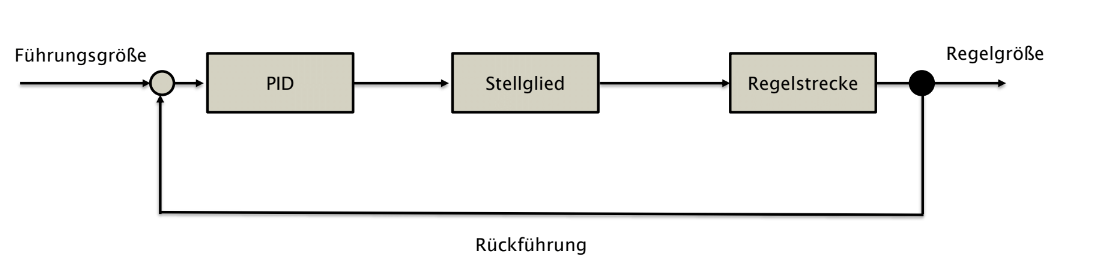
\includegraphics[scale = 0.4]{pics/Regelung}
	\caption{Blockschaltbild einer Regelstrecke}
	\label{Regelung}
\end{figure}

Eine Regelung beschreibt einen Vorgang bei dem kontinuierlich eine zu regelnde Größe erfasst und mit einer \textbf{Führungsgröße}(Sollwert) verglichen wird.
Die Differenz zwischen der gemessenen Eingangsgröße und dem Sollwert bezeichnen man als \textbf{Regeldifferenz}. 
Der PID Regler erfässt diese Differenz und berechnet damit eine allgemeine \textbf{Stellgröße}.
Mögliche Beispiele für Stellgrößen wären Motorstellungen oder die Leistung eines Heizelements.
Da das Anpassen der Stellgröße nichtlinear bzw. verzögert erfolgen kann, wird das Stellglied als eigenes Blockschaltbild mit aufgenommen. 
Das letzte Element bildet die Regelstrecke. Hier befindet sich das zu regelnde System. Um das Verhalten einer Regelung im Zusammenhang mit einem System ausreichend beschreiben zu können, ist deswegen eine genaue mathematische Beschreibung der physikalischen Vorgänge des Systems notwendig. Denn nur so kann festgestellt werden wie die Regelgröße auf Änderungen der Stellgröße reagiert.

\subsubsection{Regelung}
Ein \textbf{PID Regler} besteht hierbei aus drei Teilen.\newline
Dem \textbf{P (Proportional) Anteil}, welcher proportional zur Regeldifferenz(e(t)) die Stellgröße beeinflusst.
\begin{equation} 
P_{Out}(t) = K_P*e(t)
\end{equation}

Einem \textbf{I (Integral) Anteil}, der das Integral der Regeldifferenz bildet und dadurch den Regler mit einer Art Gedächtnis ausstattet. Sollte bei gleicher Stellgröße eine Differenz zwischen Führungsgröße und Regelgröße über einen längeren Zeitraum vorhanden sein, erhöht der I-Anteil weiterhin die Stellgröße. Bei einem Regler der nur aus einem K-Anteil besteht könnte es so zu einer bleibenden Regeldifferenz kommen.

\begin{equation} 
I_{Out}(t) = K_I*\int_0^t e(t') dt'
\end{equation}

Und einem \textbf{D (Derivative) Anteil}, welcher kontinuierlich die Änderungsrate der Regeldiffernz bestimmt. Dadurch kann der Regler auf schnelle Änderungen der Regelgröße reagieren.

\begin{equation} 
D_{Out}(t) = K_D*\frac{e(t)}{dt}
\end{equation}

Jede der Komponenten liefert einen Betrag zur Ausgabegröße des PID Reglers. Je nach Anwendung ist jedoch eine andere Dimensionierung der Konstanten Faktoren notwendig, um so den Einfluss auf die Ausgabestellgröße des Reglers zu bestimmen.

\begin{equation} 
Stellgroesse(t) = P_{Out}(t) + I_{Out}(t) + D_{Out}(t)
\end{equation}

\subsubsection{Model}
Um die Konstanten des Reglers bestimmen zu können, wird ein Modell erstellt. Dafür muss zuerst das zu regelnde System mathematisch beschrieben werden. Denn nur so kann die Reaktion eines Systems auf Stellgrößenänderungen simuliert werden. Die Regelstrecke bildet eine gleichförmige Kugel mit Radius \(r_{Kugel}\) auf einer schiefen Ebene.
Die Parameter sind folgende:
\begin{itemize}
\item Führungsgröße: Gewünschte Position der Kugel.
\item Stellgröße: Neigung der Platte.
\item Regelgröße: Aktuelle Position der Kugel.
\end{itemize}

Da die Regelung in X- und in Y- Richtung jeweils analog erfolgt reicht es das System in nur eine Richtung zu betrachten. Es wurde angenommen, dass zu keinem Zeitpunkt eine Gleitbewegung der Kugel stattfindet sondern eine Haftreibung auf die Kugel wirkt. Außerdem wird eine konstante Massenverteilung der Kugel angenommen.
Die Beschleunigung ergibt sich aus der von der Kugelmasse abhängigen Gewichtskraft \(F_G\) und der daraus resultierenden Hangabtriebskraft \(F_{Hang}\) bei einem Plattenneigungswinkel \(\phi\).

\begin{equation} 
F_{Hang} = m_{Kugel} * g * \sin\phi
\label{eq:Hangabtrieb}
\end{equation}

Die translatorische Beschleunigung, des Massenmittelpunkts der Kugel, entlang der X-Achse kann durch Anwendung des 2. Newton'schen Axioms berechnet werden.

\begin{equation} 
\sum{F_{Ext}} = m_{Kugel} * \ddot{x}
\end{equation}

\begin{equation} 
F_{Hang} + F_{Haftreibung} = m_{Kugel} * \ddot{x}
\end{equation}

\begin{equation} 
F_{Haftreibung} = m_{Kugel} * \ddot{x} - F_{Hang}
\label{eq:Haftreibung} 
\end{equation}

Sie \(I_{Kugel}\) das Trägheitsmoment einer homogenen Kugel, \(M_{Ext}\) ein auf die Kugel wirkendes Drehmoment  und \(\alpha\) der Drehwinkel. Die Anwendung des 2. Newton'schens Axioms für Drehbewegungen ergibt:
\begin{equation} 
\sum{M_{Ext}} = I_{Kugel} * \ddot{\alpha}
\end{equation}

\begin{equation} 
-F_{Haftreibung} * r_{Kugel} = I_{Kugel} * \ddot{\alpha}
\label{eq:Drehbewegung}
\end{equation}

Die Beschleunigungen(Translation und Rotation) stehen über die Rollbedingung im Zusammenhang.

\begin{equation} 
\ddot{x} = \ddot{\alpha} * r_{Kugel}
\end{equation}

\begin{equation} 
\ddot{\alpha} = \frac{\ddot{x}}{r_{Kugel}}
\label{eq:Winkelbeschleunigung}
\end{equation}

Durch einsetzen der Gleichungen \ref{eq:Hangabtrieb}, \ref{eq:Haftreibung} und \ref{eq:Winkelbeschleunigung} in Gleichung \ref{eq:Drehbewegung} erhält man:

\begin{equation} 
(m_{Kugel} *  g *\sin\phi * r_{Kugel} - m_{Kugel} * \ddot{x}) = I_{Kugel} * \frac{\ddot{x}}{r_{Kugel}}
\end{equation}

\begin{equation} 
g * \sin\phi - \ddot{x} = I_{Kugel} * \frac{\ddot{x}}{m_{Kugel} * r_{Kugel}^2}
\end{equation}

\begin{equation} 
\ddot{x} =  \dfrac{g * \sin\phi }{1 + \dfrac{I_{Kugel}}{m_{Kugel} * r_{Kugel}^2}}
\label{eq:Kugelbeschleunigung}
\end{equation}

Das Trägheitsmoment einer homogenen Kugel ist:

\begin{equation} 
I_{Kugel} =  \frac{2}{5} * m_{Kugel} * r_{Kugel}^2
\end{equation}

Setzt man dies nun in Gleichung \ref{eq:Kugelbeschleunigung} ein, folgt daraus eine Differenzialgleichung 2. Ordnung, welche die Kugelbeschleunigung bei einer gegenbenen Plattenneigung \(\phi\) beschreibt.

\begin{equation} 
\ddot{x} =  \dfrac{5}{7}*g* \sin\phi
\end{equation}

\begin{figure}[htb]
	\centering
	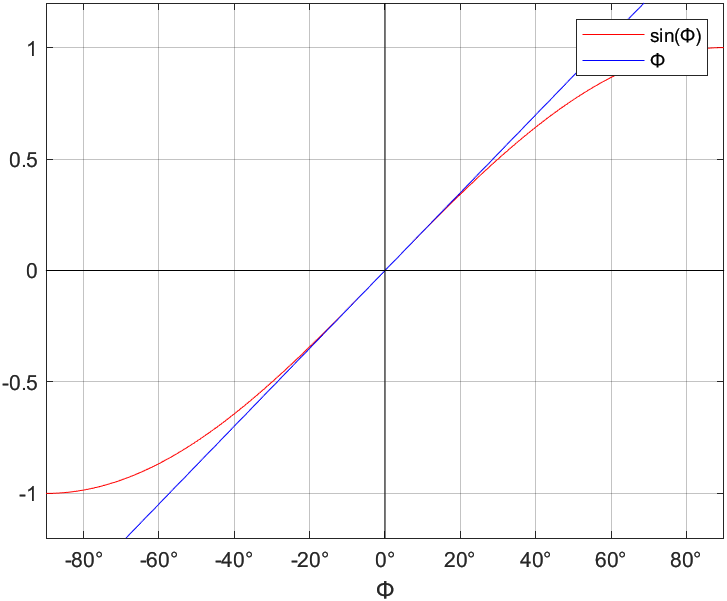
\includegraphics[scale = 1]{pics/Kleinwinkel}
	\caption{Kleinwinkelnäherung}
	\label{Kleinwinkel}
\end{figure}

Da die Auslenkwinkel der Platte sich in einem Bereich von -15 Grad bis + 15 Grad befinden, wenden wir die Kleinwinkelnäherung an und nähern \(\sin\phi\) durch \(\phi\).

Denn wie Abbildung \ref{Kleinwinkel} zeigt, besitzt die Sinusfunktion für kleine Winkel ein lineares Verhalten.

\begin{equation} 
x(t) =  \iint\dfrac{5}{7}*g* \phi dt^2
\end{equation} 

Das Lösen von Differenzialgleichungen ist häufig Aufwendig, deshalb werden diese in den Laplacebereich transformiert. Hier sind Differenzieren und Integrieren durch arithmetische Operationen möglich. Die Übertragungsfunktion einer Strecke bildet also den Quotienten aus laplacetransformierter Ausgangsfunktion und Eingangsfunktion der Regelstrecke.

\begin{equation} 
G_{Strecke} =  \dfrac{x(s)}{\beta(s)} = \dfrac{5}{7} * g * \dfrac{1}{s^2}
\end{equation}

Zur Annäherung des Verhaltens des Stellglieds(der Servomotoren und der Platte) wurde ein PT2-Glied gewählt. Jedoch erwies sich das validieren der Sprungantwort der Übertragungsfunktion als schwierig, da kein geeignetes Messverfahren für den Plattenwinkel gefunden werden konnte.

\begin{equation} 
G_{Stellglied} =  \dfrac{\beta(s)}{\beta_{soll}(s)} = 
\dfrac{K}{T^2*s^2+2*D*T*s+1}
\end{equation}

Wobei \(K\) den Verstärkungsfaktor, \(T\) die Zeitverzögerung und \(D\) den Dämpfungsgrad darstellt. Versuche das Verhalten mit einer Kamera zu messen führten zu folgenden Konstanten und letztlich der Übertragungsfunktion des Stellglieds:

\begin{equation} 
G_{Stellglied} =  \dfrac{\beta(s)}{\beta_{soll}(s)} = 
\dfrac{1}{0.0016*s^2+0.048*s+1}
\end{equation}

Multipliziert man beide Übertragungsfunktionen miteinander ergibt das die Funktion des Systems. Diese bildet die Grundlage für die Bestimmung der PID-Reglerkonstanten. 

\begin{equation} 
G_{System} = \dfrac{5}{7} * 9.81 * \dfrac{1}{s^2} * \dfrac{1}{0.0016*s^2+0.048*s+1}
\end{equation}
\begin{equation} 
G_{System} = \dfrac{7.0071}{{(0.0016*s^2+0.048*s+1)*s^2}}
\end{equation}

Damit wurde ein Matlabscript erstellt, das mithilfe der Übertragungsfunktion und dem Tool PID Tuner eine Anpassung der Reglerkonstanten ermöglicht. Das Ergebnis sind die Werte:

\begin{itemize}
\item \(K_P\): 1.04
\item \(K_I\): 0.14
\item \(K_D\): 0.56
\end{itemize} 

\begin{figure}[htbp]
	\centering
	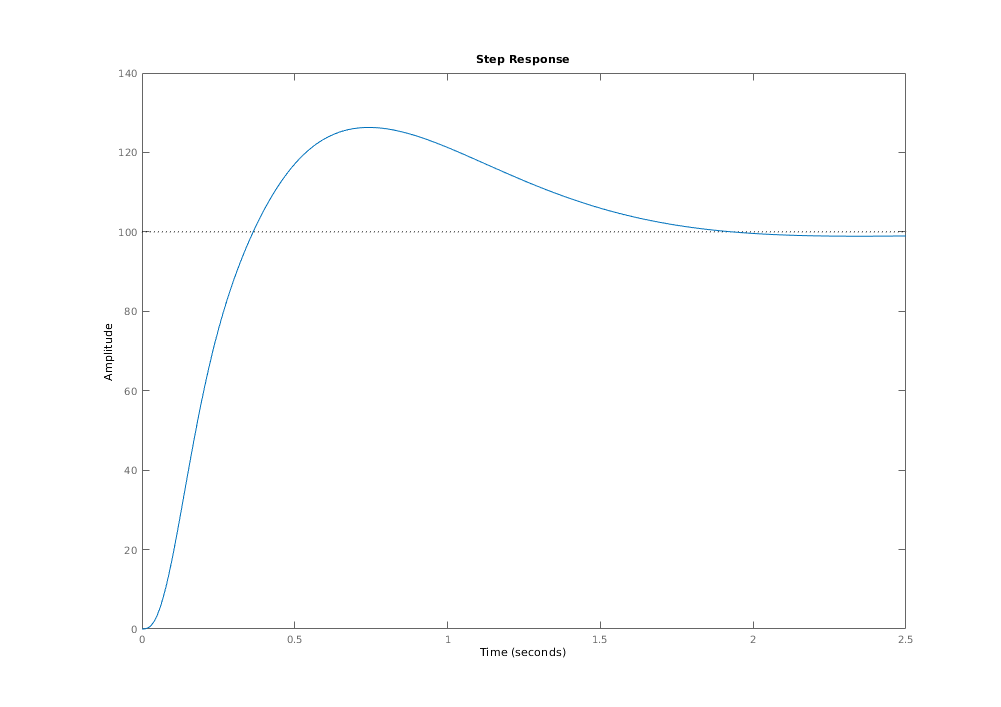
\includegraphics[scale = 0.35]{pics/Sprung}
	\caption{Sprungantwort des Systems}
	\label{Sprung}
\end{figure}

Ein Führungsgrößensprung von X-Koordinate 0 zu 100 führt dann zu der in Abbildung \ref{Sprung} gezeigten Sprungantwort.

Leider erwiesen sich die berechneten Werte als nicht praxistauglich. Mögliche Gründe hierfür könnten eine falsche Abschätzung des Stellglieds sein oder die Tatsache, dass durch das Ändern des Neigungswinkels eine zusätzliche Kraft auf die Kugel wirkt wenn sich diese nicht im Mittelpunkt der Platte befindet.\newline
Deswegen wurde ein empirisches Verfahren zur Bestimmung der Regelparameter verwendet. Hierbei wird zuerst \(K_P\) auf einen unkritischen Wert und \(K_P\) bzw. \(K_P\) auf 0 gestellt. Schrittweise erhöht man nun \(K_P\) bis das System anfängt zu schwingen. Danach reduziert man \(K_P\) wieder etwas und erhöht die beiden anderen Konstanten bis ein akzeptables Ergebnis erzielt wird. 

\subsubsection{Verbesserungen}
Durch die Einstellung des Plattenneigungswinkels mittels drei Servomotoren könnte man den Neigungswinkel nicht mehr am Plattenmittelpunkt angreifen lassen sondern an der Kugelposition. Das hätte zur Folge, dass die Kraft die auf die Kugel beim Ändern des Winkels wirkt, nicht zustande kommt.\newline
Mithilfe eines geeigneten Messverfahrens für den Plattenneigungswinkel könnte man auch die Übertragungsfunktion des Stellglieds verifizieren und so die Annäherung durch das Modell verbessern.
Sollte dies keine Besserung bringen gibt es auch noch andere empirische Verfahren um Reglerwerte zu bestimmen. (Ziegler/Nichols oder Chien, Hrones und Reswick)

% ----------------------------------------------------------------------------------
% Kapitel 2.7: PWM Signale
% ----------------------------------------------------------------------------------
\subsection{PWM-Signale}
\textit{Von Michael Braun und Michael Schmidt}\newline
\subsubsection{ Allgemeines}
Die Ansteuerung der Servomotoren erfolgt über ein 50 Hz PWM-Signal, welches mittels der Funktion 
"`PWM\_SetDutyCycle"\, auf die jeweils aktuellen Werte geändert wird. Diese Funktion wandelt automatisch 
die Werte die im Promillebereich, im Format $0-10000$, angegeben werden, in die richtige Länge des 
Hochanteils des PWM-Signals um. Diese Funktionen werden von den Dave 4- eigenen APPs zu Verfügung 
gestellt. Dabei sind durch die Servomotoren einige Werte vorgegeben:

\begin{tabularx}{\textwidth}{p{0.25\textwidth}|X|X|X|X|X|}
\hline
 Bezeichnung 		& Wert in ms (zu 20ms/50Hz) & Wert in Prozent 	& Wert in Promille \\
\hline
 Minimalstellung		& 0,9						& 4,5				& 450 \\
\hline
 Neutralstellung		& 1,5						& 7,5				& 750 \\
\hline
 Maximalstellung		&2,1						& 10,5				& 1050\\
\hline
%\caption{Tabelle: Werte der Servomotoren}
%\label{servowerte}
\end{tabularx}
\newline
Sollten die übertragenen Werte den Maximalwert von 1050 überschreiten, werden sie lediglich auf den 
Maximalwert gesetzt, um eine korrekte Ansteuerung der Servomotoren zu gewährleisten. Diese Werte werden 
kontinuierlich von der Regelung verändert und über die Pins 3.0, 3.3 und 3.4 des XMC an die Servomotoren 
ausgegeben. Dies wird in einem Interrupt abgearbeitet, das im 50 Hz Takt aufgerufen wird. Dabei sind jedoch 
noch motorenspezifische Unterschiede aufgetreten, die in Tabelle 3 aufgeführt werde. Diese sind nötig, um 
die Platte initial in eine ebene Nullstellung zu positionieren.

\begin{tabularx}{4cm}{|l|l|}
\hline
 Servomotor		& Offset \\
\hline
 1				& 35	\\
\hline
 2				& 15\\
\hline
 3				& 5	\\
\hline
%\caption{Tabelle: Werte der Servomotoren}
%\label{offsets}
\end{tabularx}
\newline
\subsubsection{Probleme und Ausblick}

Jedoch wird die Auslenkung der Hebel durch die Aufhängung der Motoren begrenzt, da ab einem 
bestimmten Wert die Platte an diese stößt. Dadurch ergeben sich folgende Einschränkungen:
\newline
\begin{tabularx}{8cm}{|l|l|l|}
\hline
 Servomotor		& Minimalwert & Maximalwert \\
\hline
 1				& 600		&  1050 \\
\hline
 2				& 490		& 950\\
\hline
 3				& 490		& 950\\
\hline
%\caption{Tabelle: Werte der Servomotoren}
%\label{einschränkungen}
\end{tabularx}
\newline
Der Maximalwert ergibt sich dabei aus dem Umstand, dass die Hebel in der Verbindung zwischen Motor und 
Dreiecksverbindung überdrehen und dadurch die Platte eher absenken als sie auf ihre maximale Auslenkung zu 
bringen. 
 \begin{figure}[htbp]
	\centering
	
\includegraphics[scale = 0.8]{pics/neuedreiecksverbindung}
	\caption{Aufbau einer alternativen Dreiecksverbindung mit größerem Wirkungsradius}
	\label{fig:dreieckneu}
\end{figure}
Dieses Problem könnte dabei in Zukunft mittels einer neuen Dreiecksverbindung gelöst werden, die auch niedrigere 
Auslenkungen erlaubt \ref {fig:dreieckneu}. Leider kamen wir aufgrund von Zeitdruck nicht mehr dazu diese neue Verbindung zu drucken. 
Allerdings wäre auch noch die Befestigung an der Platte ein Problem, da die alte Verbindung bereits mittels Silikon befestigt und 
eine Beschädigung beim Ablösen dieser zu befürchten war. Glücklicherweise hat der Regler solche extremen Ausschläge auch gar nicht zu 
handhaben, da die Regelung für unsere Zwecke ausreichend Spielraum zum balancieren hat.


\subsubsection{Fazit}
Abgesehen von Anfangsschwierigkeiten mit dem Flashen des XMCs, war die Ansteuerung über PWM-Signale 
mit den internen Dave 4 APPs sehr einfach zu lösen, wobei natürlich auch das verspätete Auffinden der Dokumentation dieser APPsmit hineingespielt hat. 
Lediglich die Berechnung bzw. das Ausprobieren der mechanischen Einschränkungen und die korrekte Übergabe der Werte durch UART stellten eine kleine Herausforderung dar. 

% ----------------------------------------------------------------------------------
% Kapitel 2.8: Threading auf dem Raspberry Pi
% ----------------------------------------------------------------------------------
\subsection{Threading auf dem Raspberry}
\textit{Von Korbinian Federholzner}\newline
Das erhalten der UDP-Packete und der UART-Frames, wurde in Blocking-Loops implementiert, dadurch wäre die Anwendung 
die ganze Zeit durch diese Loops blockiert. Um dieses Verhalten zu umgehen wurden alle Listening-Loops in eigene Threads
verschoben. Da die Anwendung zentral von einem Button gesteuert wird, welcher zwischen den Modus zum Regeln und dem 
Modus zur manuelle Steuerung mit der App wechselt, gesteuert wird, befindet sich die Ansteuerung des Buttons im main Thread.
Für den Regeler und das manuelle Ansteuern gibt es auch wieder zwei Threads welche je nach Zustand des Buttons auf 
aktiv gesetzt werden. Um den Zugriff auf die gelesenen Daten von UART und UDP sicher zu gewährleisten, wurde mittels 
Mutex der Zugriff auf die Daten abgesichert. Dabei kann nur entweder UART schreiben oder der Benutzer die Daten abfragen,
niemals beide gleichzeitig.


% ----------------------------------------------------------------------------------
% Kapitel 2.9: UDP-Socket
% ----------------------------------------------------------------------------------
\subsection{UDP-Socket}
\textit{Von Patrick Lesch}\newline
Zum externen Empfang von Steuersignalen wurde auf dem Raspberry Pi ein UDP-Socket implementiert welcher auf eingehende Daten auf
Port 1337 wartet. Dieser Port wurde festgelegt um den Kommunikationsaufbau zu vereinfachen und Störquellen zu minimieren. Durch 
einen festgelegten Port wird sichergestellt, dass keine ungewollten Nachrichten auf eventuell bereits belegten Ports eingehen und die 
Kommunikation erschweren. Zur Verbindung wird vorausgesetzt, dass sich die Geräte im selben Netzwerk befinden und dieses die Kommunikation
zwischen den Geräten zulässt. Im Gegensatz zu anderen Protokollen erfüllt UDP am besten die Echtzeitanforderungen des Projekts da stets
die aktuellsten Daten gesendet werden. 

Zusätzlich zur iOS-Applikation können durch den UDP-Socket auch andere Geräte mit dem Raspberry Pi kommunizieren. Die Funktionalität kann so
beliebig erweitert werden. Während der Recherche zu sinnvollen Echtzeitübertragungen wurde unter anderem in Erwägung gezogen die Kommunikation
über Bluetooth statt Wlan stattfinden zu lassen. Dies hätte zwar potentiell geringere Latenzen aber auch einen begrenzten Raum zur Steuerung gebracht.
Dank der Kommunikation über das Netzwerk kann die Platte auch aus weiter Entfernung bedient werden ohne, dass merkliche Verzögerungen eintreten. 
Eine weitere Überlegung stellten andere Protokolle wie Beispielsweise TCP dar. Diese waren für das Projekt aufgrund eines potentiellen Kommunikationsstaus 
ungeeignet, da die App dann auf eine Bestätigung des Raspberry Pi warten müsste. Somit wäre nicht gewährleistet, dass stets die aktuellsten Daten
empfangen werden. Ein eigener Hotspot wurde aus Gründen der Bürokratie als Idee verworfen, da die Hochschule diesen erst speziell genehmigen müsste.

% ----------------------------------------------------------------------------------
% Kapitel 2.10: IOS-Appliaktion
% ----------------------------------------------------------------------------------
\subsection{iOS-Applikation}
\textit{Von Patrick Lesch}\newline

\subsubsection{Allgemeines}
Eine der Anforderungen an das Projekt war, dass die Platte manuell steuerbar sein sollte. Dazu wurde eine Applikation für 
iOS-Geräte entwickelt. Ziel der Applikation ist es die Neigung des mobilen Endgerätes an den Raspberry Pi zu übertragen. 
Dieser übersetzt die übermittelten Werte in Neigungswinkel mit deren Hilfe der XMC die Motoren ansteuert welche die Platte 
in eine Lage versetzen welche die Lage des iOS-Gerätes spiegelt.

Um eine möglichst einfache und Geräteübergreifende Installation auf verschiedenen Geräten zu gewährleisten wurde erwogen die App 
als Webapp zu implementieren. Dieser Ansatz wurde aufgrund von in iOS 13 von Apple eingeführten Policies verworfen. Die Abfrage zur Genehmigung
des Auslesens des Gyroskops muss für verschiedene iOS Versionen aktuell unterschiedlich implementiert werden. Das hätte einen für das Projekt
unverhältnismäßigen Mehraufwand bedeutet der den zeitlichen Rahmen des Projekts gesprengt hätte. 

Ein weiteres Gegenargument stellte zudem die durch den Browser festgelegte Orientierung der Seite dar. 
Wird das Gerät gedreht während die Orientierung des Gerätes entsperrt ist dreht sich dieser entsprechend mit. 
Dies würde bei jedem Kippen des Gerätes den Browser drehen was wiederum die zu übertragenden X- und Y-Winkel des Gerätes drehen würde. 
Durch eine native Implementierung als iOS-App kann gewährleistet werden, dass die Orientierung der App immer festgesetzt ist und die Daten 
unabhängig von Systemweit aktivierter Orientierungssperre gleich bleibt.

\subsubsection{Views}
Die Applikation verfügt im wesentlichen über zwei Views. Der erste View der nach dem Splash-Screen gestartet wird ist der QR-Scanner. 
Wird ein QR-Code erfolgreich gescannt wird zum eigentlichen Steuerungs-View gewechselt welcher die Winkel der X- und Y-Achse, sowie 
die IP die mittels QR-Code eingelesen wurde anzeigt.

\subsubsection{Implementierung}
Umgesetzt wurde die App zum großteil in nativem Swift-Code. Für den Aufbau der UDP-Verbindung und dem einrichten des sendenden Sockets
werden Apples C Libraries verwendet. Als Verbindungsart zwischen iOS-App und Raspberry Pi wurde UDP gewählt um eine Echtzeitübertragung zu garantieren. 
Da die App dank UDP kein Acknowldge des Raspberry Pi erwartet gibt es weder Verzögerung noch einen Datenrückstau. Gegebenenfalls bei
der Übertragung verlorengegangene Daten wurden in Kauf genommen um stets möglichst aktuelle Werte an die Platte zu liefern. 

Da der Raspberry Pi, wie in Kapitel 2.9 erwähnt, auf Port 1337 lauscht sendet die App nur auf diesem ihre X- und Y-Winkel. Die Winkel werden 
von der iOS-Schnittstelle die das Gyroskop des Gerätes ausliest in Radiant angegeben. Vor der Übertragung werden diese aufbereitet indem
sie in Grad umgerechnet und auf 3 Nachkommastellen gerundet werden. Zusätzlich werden diese Werte mit einem Faktor von 0.5 multipliziert, da sich
gezeigt hat, dass die Bewegung der Platte die notwendig ist um die Kugel zu bewegen kleiner ist als die Neigung die ein Nutzer sinnvoll steuern kann. 
Ohne diese Ergänzende Anpassung reichten bereits minimale Bewegungen um die Platte stark zu bewegen was ein Kontrollieren der Kugel schwierig machte.

Die aufbereiteten Winkel werden zur Übertragung an die Sende-Funktion als String in dem Format 
"`X\_ACHSEN\_WINKEL;Y\_ACHSEN\_WINKEL;"\ übergeben welche diesen über den festgelegten Port an die gescannte IP überträgt.
Auf dem Raspberry Pi kann anhand der Semikola zwischen den einzelnen Winkeln einer Nachricht unterschieden werden. 
Das Aktualisierungsintervall des Gyroscops wurde aufgrund guter Ergebnisse auf 60 Hz festgelegt. 

% ----------------------------------------------------------------------------------
% Kapitel 2.11: Zusammenführung
% ----------------------------------------------------------------------------------
\subsection{Zusammenführung der einzelnen Komponenten}
Diverse Probleme gab es beim Merge-Vorgang auf Gitlab mit den durch Dave4 automatisch erstellten Files. 
Diese erfassen die konfigurierten Einstellungen der XMC APPs und überführen diese in ausführbaren Code. 
Dieses Problem wurde dadurch gelöst, dass man die Einstellungen auf einem Branch durchgeführt hat und 
lediglich die selbstgeschriebenen Code-Files zusammengeführt hat. Im Bereich der App gestaltete sich das 
Zusammenführen der Komponenten dank guter Zusammenarbeit denkbar einfach und es traten an dieser Stelle 
keine unvorhergesehenen Fehler auf.

\pagebreak
% ----------------------------------------------------------------------------------
% Kapitel 3: Benutzerhandbuch
% ----------------------------------------------------------------------------------
\section{Benutzerhandbuch}
\subsection{Starten des Prototyps}
%TODO ALLE!
Schritt 1:
Einloggen mit Benutzername "`pi"\ und Passwort "`raspberry"\
\newline
Schritt 2: Aufrufen des QR-Codes mit Hilfe des folgenden Kommandos: 
\newline(die inneren \"\, gehören zum Befehl)
\newline\newline
"`raspberry"\ "`hostname -I | awk '{print \$1}' | qr \&\& hostname -I | awk '{print \$1}' | xargs echo "`BalancingPlate IP: \$1"\,"\,
\newline\newline
    (Ein QR Code sowie der Text "`BalancingPlate IP: $<$RaspberryPi-IP$>$"\,) sollte ausgegeben werden.)
\newline
Schritt 3:
%TODO Korbinian

\subsection{Flashen des Custom-Kernels und allgemeine Einrichtung}
%TODO Patrick Lesch
Alle Kommandos sind im folgenden zwischen doppelten Anführungsstrichen: "`command"\,

1. Raspbian Buster Lite herunterladen.
   https://www.raspberrypi.org/downloads/raspbian/
\newline

2. Auf die SD-Karte flashen (z.B. mit BalenaEtcher unter Windows)\newline
   https://www.balena.io/etcher/
\newline

3. Raspberry-Pi booten und einrichten:
\newline
3.1 Login: "`pi"\, | Passwort: "`raspberry"\, (Achtung! Englisches Layout standardmäßig --$>$ y == z und umgekehrt)\newline
3.1.x1 Nach dem Bootvorgang ist der Bildschirm schwarz:\newline
3.1.x2 SD-Karte in PC stecken und in der Config.txt unter [pi4] "`dtoverlay=vc4-fkms-v3d"\, mit "`\#"\, auskommentieren.
       (Das erzwingt Legacy Treiber.) Falls das nichts bringt - google is your friend.
\newline
3.2 Config anpassen: "`sudo raspi-config"\,\newline
3.2.1 WLAN einrichten: Network Options (Dort dem Dialog folgen und die Verbindung einrichten)\newline
      [Verbindung prüfen. z.B. mit "`ping google.com"\, oder mit "`ifconfig"\,]\newline
3.2.2 SSH einschalten: Interfacing Options --$>$ SSH\newline
3.2.3 Neustart: "`sudo reboot"\,\newline
\newline
4. Preempt-RT Kernel flashen:\newline
4.1 Dem Tutorial hier folgen und Kernel selber kompilieren\newline
    https://lemariva.com/blog/2019/09/raspberry-pi-4b-preempt-rt-kernel-419y-performance-test
    oder den fertigen aus dem Git-Repository nehmen [Für den Raspberry Pi 4B "`kernel\_4\_19\_59-rt23-v7l+"\, nehmen (siehe Tutorial-Link)]
    https://github.com/lemariva/RT-Tools-RPi/tree/master/preempt-rt\newline
4.2 Den Kernel an den Raspberry senden: "`scp rt-kernel.tgz pi@$<$ipaddress$>$:/tmp"\,\newline
4.3 Am Pi folgende Kommandos ausführen um den Kernel zu entpacken und einzurichten:\newline
\begin{itemize}
    \item "`cd /tmp"\,
    \item "`tar xzf rt-kernel.tgz"\,
    \item "`cd boot"\,
    \item "`sudo cp -rd * /boot/"\,
    \item "`cd ../lib"\,
    \item "`sudo cp -dr * /lib/"\,
    \item "`cd ../overlays"\,
    \item "`sudo cp -d * /boot/overlays"\,
    \item "`cd .."\,
    \item "`sudo cp -d bcm* /boot/"\,
\end {itemize}

4.4 Config.txt bearbeiten um den neuen Kernel zu nutzen:\newline
4.4.1 Mit nano öffnen: "`sudo nano config.txt"\,\newline
4.4.2 An das Ende folgendes einfügen: "kernel=kernel7\_rt.img"\,\newline
4.4.3 Reboot ("`sudo reboot"\,)\newline
4.4.4 Prüfen ob der Kernel funktioniert: "`uname -r" \,sollte "`4.19.59-rt23-v7l+"\, ausgeben. 
      (Die Version die man kompiliert hat)\newline
\newline

5. UART einschalten:\newline
5.1 Config.txt mit nano öffnen: "`sudo nano config.txt"\,\newline
5.2 An das Ende folgendes einfügen: "`enable\_uart=1"\,\newline
5.3 Reboot ("`sudo reboot"\,)\newline
\newline
6. Kleines Raspberry Pi Display des Hardware-Kartons rotieren:\newline
6.1 Config.txt mit nano öffnen: "`sudo nano config.txt"\,\newline
6.2 An das Ende folgendes einfügen: "`display\_rotate=2"\,\newline
6.3 Reboot ("`sudo reboot"\,)\newline
\newline
7. Software installieren / updaten:\newline
7.1 "`sudo apt update"\,\newline
7.2 "`sudo apt install pip"\,\newline
7.3 QR installieren: "`pip install qrcode[pil]"\,
    (https://github.com/lincolnloop/python-qrcode)\newline
7.4. WiringPI: "`sudo apt install wiringpi"\ \newline
7.5. "`sudo apt install cmake"\ \newline

8. Starten des Programmes \newline
8.1 Navigieren in das Verzeichnis in dem CMakeList.txt liegt \newline
8.2 "`cmake ."\ \newline
8.3 "`make"\ \newline
8.4 danach sollte eine Executable in /bin liegen 


\subsection{Bekannte Probleme}
%TODO ALLE!
\begin{itemize}
    \item Wurde mittels QR-Code eine falsche IP gescannt muss die App neu gestartet werden\,
\end {itemize}


\pagebreak
% ----------------------------------------------------------------------------------
% Kapitel 4: Fazit/Zusammenfassung
% ----------------------------------------------------------------------------------
\section{Fazit}
Das Projekt wurde fristgemäß mit allen daran festgelegten Anforderungen abgeschlossen. Es befindet sich in einem 
funktionsfähigen und erweiterbarem Zustand. Dennoch besteht weiteres Verbesserungspotential. So könnte etwa die 
derzeit noch langsame und etwas ruckelige Regelung optimiert werden. Des weiteren könnten weitere Funktionen eingebaut werden. 
Wünschenswert wäre hier etwa die graphische Ausgabe der aktuellen Kugelposition in der iOS-App oder das festlegen eines Punktes auf
dem iOS-Geräte Display welches die Kugel analog auf die entsprechende Position der Platte bringt. Dadurch könnten auch noch gewisse 
Formen nachgefahren werden (z.B. ein Unendlichkeitszeichen).
\newline
Insgesamt kann das Projekt dennoch als Erfolg betrachtet werden, da ein funktionsfähiger Prototyp mit kleineren Fehlern geschaffen wurde, 
der ein großes Erweiterungspotential besitzt und außerdem für Vorführungen zur verfügung steht.

\pagebreak



% ----------------------------------------------------------------------------------------------------------
% Anhang
% ----------------------------------------------------------------------------------------------------------
\pagenumbering{Roman}
\setcounter{page}{1}
\lhead{Anhang \thesection}

\begin{appendix}
\section*{Anhang}
\phantomsection
\addcontentsline{toc}{section}{Anhang}
\addtocontents{toc}{\vspace{-0.5em}}


\end{appendix}

% ----------------------------------------------------------------------------------------------------------
% Abbildungsverzeichnis (optional)
% ----------------------------------------------------------------------------------------------------------
\section {Abbildungsverzeichnis}
\listoffigures
\pagebreak

% ----------------------------------------------------------------------------------------------------------
% Tabellenverzeichnis (optional)
% ----------------------------------------------------------------------------------------------------------
\listoftables
\pagebreak


% ----------------------------------------------------------------------------------------------------------
% Literatur
% ----------------------------------------------------------------------------------------------------------
\renewcommand\refname{Literaturverzeichnis}
\lhead{}
%\bibliographystyle{alpha}
\bibliographystyle{ieeetr}
\bibliography{quellen}
\pagebreak

\section {Bestellliste}
%\begin{tabularx}{\textwidth}{p{0.25\textwidth}|l|l|l|l|l|X|}
%\hline
% Produktname					& Produkt Nr.			& Kosten				& Stück  &Gesamtkosten &Link \\
%\hline
% Servomotoren	&209913-62 &\euro{25,90} &3 &\euro{77,70}	&https://www.conrad.de/de/p/hitec-standard-servo-hs-5485hb-digital-servo-getriebe-material-karbonite-stecksystem-jr-209913.html \\
%\hline
% Servo-Hebel &1530677-VQ &\euro{6,99} &3 & \euro{20,91} &https://www.conrad.de/de/p/reely-alu-servohebel-geklemmt-47-mm-passend-fuer-futaba-servohebelkranz-anzahl-bohrungen-5-1530677.html \\
%\hline
% Gabelkopf &239186-62 &\euro{7,55} & 3 &\euro{22,65} &https://www.conrad.de/de/p/modelcraft-aluminium-gabelkopf-mit-innengewinde-m3-5-st-239186.html \\
%\hline
% Kugelgelenk &221868-62 &\euro{6,71} &3 &\euro{20,13} &https://www.conrad.de/de/p/modelcraft-stahl-kugelkopf-mit-aussengewinde-m3-1-st-221868.html \\
%\hline
% Bildschirm &1503822-62 &\euro{43,99} &1 &\euro{43,99} &https://www.conrad.de/de/p/joy-it-rb-lcd5-touchscreen-modul-12-7-cm-5-zoll-800-x-480-pixel-passend-fuer-raspberry-pi-inkl-touchpen-1503822.html \\
%\hline
% Touch-Folie &710-5240 &\euro{99,73} &1 &\euro{99,73} &https://de.rs-online.com/web/p/touchscreen-sensoren/7105240/ \\
%\hline
%\hline
% Gesamt: & & & &\euro{285,17} & \\
%\hline
%\caption{Tabelle: Bestellliste}
%\label{tbl:bestellliste}
%\end{tabularx}

\begin{figure}[htbp]
	\centering
	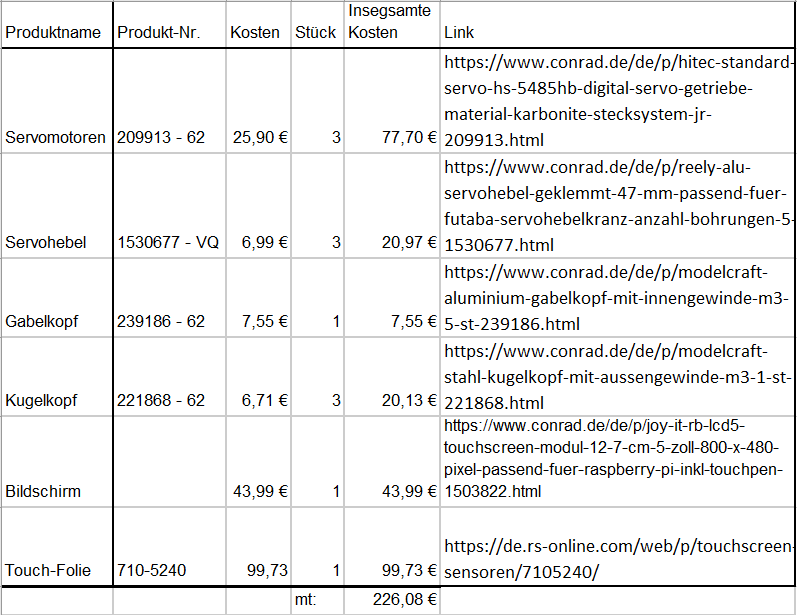
\includegraphics[scale = 0.8]{pics/Bestelliste}
	\caption{Bestellliste und Kosten des Projektes}
	\label{fig:bestell}
\end{figure}
\pagebreak

\section {Stundenliste}

\begin{table}[htb]
\centering
\begin{tabular}{|c|c|c|c|c|}
\hline
 Name					& Gesamt &Aufgabe 1	&Aufgabe 2	&Aufgabe 3 \\
 \hline
 Michael Braun			&125			&Phys. Aufbau 35			&PWM-Signale 20			&Reglerentwicklung 70			\\
 \hline
 Korbinian Federholzner	&128			&lirem ipso lorem			&lirem ipso lorem			&lirem ipso lorem			\\
 \hline
 Philipp Kramer			&123			&Touch-Folie 63			&Testing 19		&Reglerentwicklung 41			\\
 \hline
 Patrick Lesch			&125			&lirem ipso lorem			&lirem ipso lorem			&lirem ipso lorem			\\
 \hline
 Michael Schmidt		&122			&UART 62			& Phys. Bau 40			&PWM-Signale 20			\\
  \hline
\end{tabular}
\label{tab:stundenliste}
\end{table}

\end{document}
